\documentclass[a4paper,11pt]{article}
\usepackage{multicol}
\usepackage{amssymb}
\usepackage{booktabs} % For penere tabeller
\usepackage{caption} % For å legge til figurtekst
\usepackage{amsmath}
\usepackage{ragged2e}
\usepackage{physics}
\usepackage{hyperref}
\usepackage{graphicx}
\usepackage{xcolor}
\usepackage{cleveref}
\usepackage{float}
\usepackage{nicefrac}
\usepackage{booktabs}
% \usepackage{minipage}
\usepackage{enumitem} % For bedre lister
% \usepackage{biblatex} % use biblatex for handling references
\usepackage{siunitx}
\usepackage{subcaption}

\usepackage[square,numbers,sort&compress]{natbib}
\bibliographystyle{unsrtnat}


\setlength{\parindent}{2em}
\setlength{\parskip}{0.75em}
\usepackage{indentfirst}
\usepackage{mhchem} 
\definecolor{teal}{rgb}{0.04, 0.73, 0.71}


\usepackage{shorthands}

\textwidth=18cm
\oddsidemargin=-1cm
\topmargin=-1cm
\textheight=22cm

\usepackage{graphicx} % Required for inserting images

\title{FYS2810 project: \\ Calibration and data analysis of the  $^{106}$Pd($p,p'\gamma)$$^{106}$Pd data set measured at the Oslo Cyclotron Lab}
\author{Hannah Westgaard}
\date{June 2026}

\begin{document}

\maketitle

\section{Introduction}
% Nuclear level densities and $\gamma$-ray strength functions are essential for understanding atomic nuclei in the transition region from order to chaos. A case where nuclear level density remains particularly uncertain is for the stable nucleus palladium-106 (\nuclide[106]{Pd}). With a re-measurement for \nuclide[106]{Pd}$(p,p'\gamma)$\nuclide[106]{Pd} with 16 MeV protons from June 2025, the intent produce the necessary excitation vs gamma energy relations to address the uncertainty of the nuclear level densities through the Oslo-method and also independently developed Shape method. Such measurements are done through the Oslo Cyclotron Lab's (OCL) ability to produce proton beams with the MC-35 Scanditronix cyclotron, to so measure inelastically scattered protons through the Silicon Ring (SiRi) and the resulting gamma rays from de-exciting \nuclide[106]{Pd} with the scintillator array OSCAR. The goal is of the project is to calibrate the resulting OSCAR data through well-known nuclear energy levels of \nuclide[27]{Al}, and calibrating SiRi though the calculated values of QKinz\cite{qkinz}. Additionally, there was a focus on familiarizing one self with root and the process of calibrating bigger datasets. 

Nuclear level densities and $\gamma$-ray strength functions are essential for understanding atomic nuclei in the transition region from order to chaos. 
Moreover, these quantities are indispensable input for nuclear reaction codes like TALYS~\cite{TALYS}, where various cross sections and reaction rates for e.g. astrophysics and medical applications can be estimated. 
However, it is well known (as shown e.g. in Refs.~\cite{Laplace2015,Larsen2016}) that calculations of radiative capture cross sections remain highly uncertain due to the large spread in the input models that are needed for the Hauser-Feshbach formalism. 

One case where the nuclear level density is  particularly uncertain, is the stable nucleus palladium-106 ($^{106}$Pd) as shown in Fig.~\ref{fig:Goriely} (taken from Ref.~\cite{Goriely2022}).
To address the large discrepancy between the models and to obtain a model-independent slope of the nuclear level density, we have re-measured $^{106}$Pd in June 2025 through the inelastic proton-scattering reaction, $^{106}$Pd($p,p'\gamma$)$^{106}$Pd with 16-MeV protons delivered by the MC-35 Scanditronix cyclotron at the Oslo Cyclotron Lab (OCL). 
Here we measured the outgoing protons with the Silicon Ring (SiRi)~\cite{Guttormsen2011} and the gamma rays from the de-exciting $^{106}$Pd nuclei with the detector array OSCAR~\cite{Zeiser2020}. 
When the data from both detector arrays are properly calibrated, we can sort the data into an excitation-energy vs. $\gamma$-energy matrix, for which we can apply the Oslo method~\cite{Guttormsen1990, Guttormsen1987, Schiller2000} and also independently the newly developed Shape method~\cite{Wiedeking2021}. With this combined analysis our goal is to strongly constrain the nuclear level density of $^{106}$Pd and be able to verify or disprove (some of) the model calculations. 

For this project, the goal is to calibrate  the individual SiRi and OSCAR detectors using the kinematics of the reaction and well-known nuclear energy levels in the calibration runs on \nuclide[27]{Al} so that all detectors are properly gain-matched. 
Then the $^{106}$Pd data will be sorted and the calibration will be validated. 
The end goal is to obtain the $^{106}$Pd excitation energy vs. gamma-energy matrix, which is the starting point of both the Oslo method and the Shape method. Additionally, there was a focus on familiarizing one self with root and the process of calibrating bigger datasets. 


\begin{figure}
    \centering
    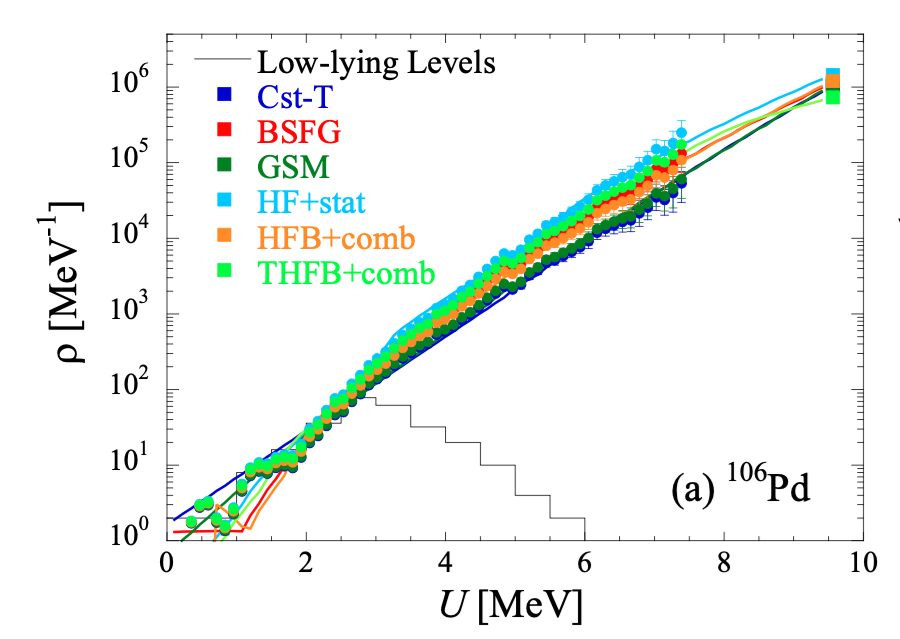
\includegraphics[width=0.5\linewidth]{figures/Fig1a_Goriely2022.png}
    \caption{The nuclear level density model of \nuclide[106]{Pd} with Oslo data. The solid black line represents the nuclear level density extracted from known discrete levels using an excitation-energy bin U = 0.5 MeV. The filled circles correspond to the Oslo data re-normalized to the corresponding theoretical model to minimize the root-mean-square deviation. The lines correspond to the six model calculations normalized to the experimental s-wave neutron resonance spacing. The full squares give the model predictions at the neutron separation energy for each of the six models.}
    \label{fig:Goriely}
\end{figure}


\newpage
\section{Experimental setup and data calibration}
\subsection{The Oslo Cyclotron laboratory (OCL)}
At the heart of the OCL is the MC-35 Scanditronix cyclotron which accelerates light ions, with proton energies ranging from 8 to 35 MeV\cite{OCL_Guttormsen}. With OSCAR and SiRi measurements enabling coincidence measurements, one can investigate reaction channels of interest through $\gamma$-decay energies and particle energies corresponding to nuclear excitation levels. 

The thickness of each target and the beam current used for each run is shown in \cref{tab:runs}. The \nuclide[106]{Pd}-target was mounted in a \nuclide[181]{Ta}-covered aluminum frame, with the tantalum's purpose being reducing reactions with \nuclide[27]{Al} in non-calibration runs. In this report the second \nuclide[106]{Pd} run and the \nuclide[27]{Al} run were used, though the data of the first run for \nuclide[106]{Pd} exists as well.

\begin{table}[]
    \centering
    \caption{All runs corresponding to this experiment were done with 16 MeV protons. The \nuclide[27]{Al}-run works as a calibration run, while the \nuclide[106]{Pd}-runs provided the data of interest. The target thickness of \nuclide[106]{Pd} is noted to be uncertain.}
    \begin{tabular}{l|c|c|c}
    \toprule
         &  \nuclide[106]{Pd} 1st run & \nuclide[106]{Pd} 2st run & \nuclide[27]{Al}\\
         \midrule
        Beam current & 0.8 - 1.3 nA & 1.5-1.6 nA & 1.3-1.8 nA \\
        Target thickness & *0.98 mg/cm$^2$ & *0.98 mg/cm$^2$ & $\sim 11 \mathrm{\mu g}$ \\ 
        \bottomrule
    \end{tabular}
    \label{tab:runs}
\end{table}
\begin{figure}
    \centering
    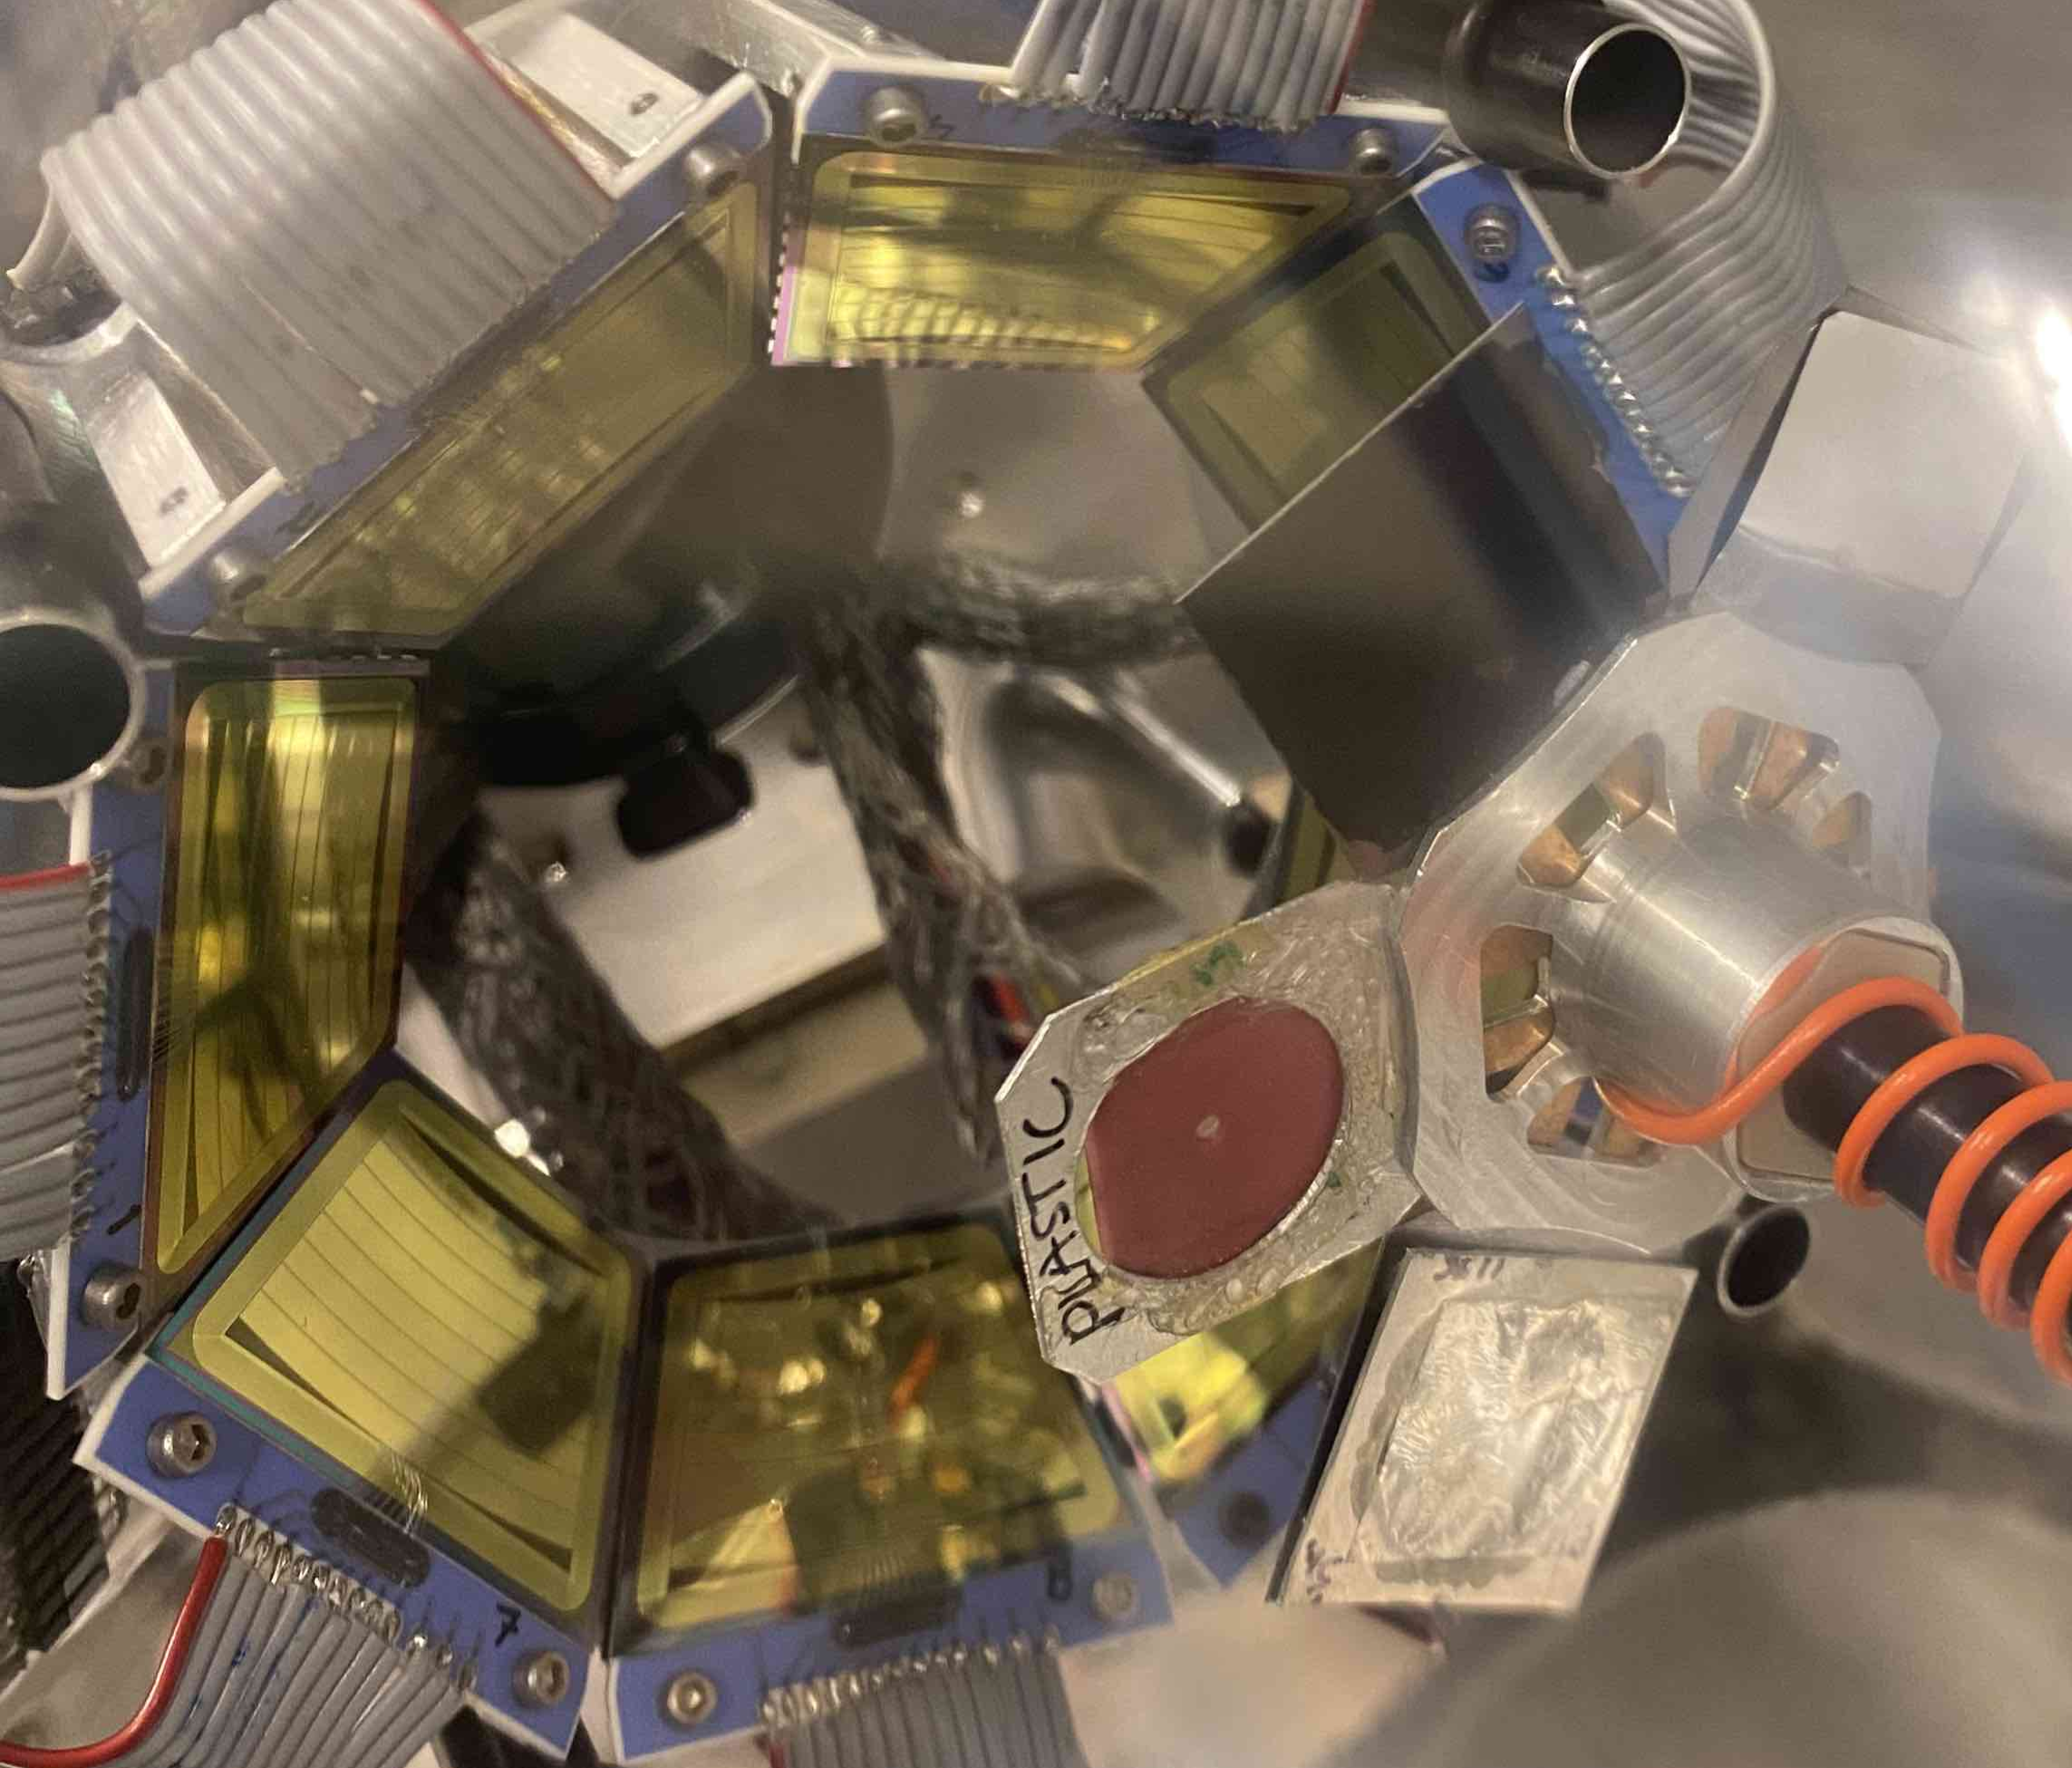
\includegraphics[width=0.5\linewidth]{figures/targets_25June2025.jpeg.png}
    \caption{Picture showing targets \nuclide[27]{Al}(position 1), \nuclide[12]{C}(position 2) and \nuclide[117]{Sn}(position 4) in the OSCAR-SiRi detection system.}
    \label{fig:targets}
\end{figure}

\subsection{Linear calibration}
For energy calibration, we have assumed a linear fit. This assumes linear detector response, appropriate for energies above $\sim$ 100 keV and below $\sim$ 3 MeV for LaBr3 \cite{LaBr3_detector_response} and light ions for SiRi \cite{LEO}. The gain $a_0$ and shift $a_1$ are determined separately dependent on detector type. $E_\text{calibrated}$ is the calibrated energy and should represent the actual energy of the $\gamma$-ray, while $E_\text{measured}$ is the raw measurement from a OCL LaBr$_3$ detector. 
\begin{equation}
    E_\text{calibrated} = a_0 + a_1\cdot E_\text{measured}
    \label{eq:linear-fit}
\end{equation}


\subsection{Particle energy detector - SiRi}
The Silicon Ring (SiRi) \cref{fig:SiRi-OSCAR} detector is a $E - \Delta E$- detector system. It is composed of 8 detector segments, with one $E$-detector and a segmented $\Delta E$ detector with 8 strips on each. In charged beam experiments, SiRi provides a typical energy resolution of 150 keV\cite{TORNYI20146}. SiRi is mounted in a backwards-angle, with angles for each strip as in \cref{tab:SiRi-angles}. During a detection event, a pulse proportional to the energy of the incoming particle is measured in both layers. Data can then be calibrated post-experiment so energy corresponding to pulses are determined using \cref{eq:linear-fit} for both $E$ and $\Delta E$ for SiRi. The gain $a_0$ and shift $a_1$ are calculated for particle x in relation to particle y (or y in relation to x if switched around) as follows:

\begin{align}
    a_0 = \frac{ E_\text{y, calculated}-  E_\text{x, calculated}}{ E_\text{y, measured}-  E_\text{x, measured}} \qquad a_1 =  E_\text{x,calculated} -(a_0\cdot  E_\text{x,measured})\label{eq:a1b1} 
\end{align}



\begin{table}[htbp]
    \centering
    \caption{Strip angles for SiRi in backwards angle. The angle represents the middle of each strip.}
    \begin{tabular}{c cccccccc}
        \toprule
        Strip & $f_0$ & $f_1$ & $f_2$ & $f_3$ & $f_4$ & $f_5$ & $f_6$ & $f_7$ \\
        \midrule
        Angle ($^\circ) \pm 2^\circ$ & 140 & 138 & 136 & 134 & 132 & 130 & 128 & 126 \\
        \bottomrule
    \end{tabular}
    \label{tab:SiRi-angles}
\end{table}

% \begin{align}
%     &a_0 = \frac{ E_\text{y, calculated}-  E_\text{x, calculated}}{ E_\text{y, measured}-  E_\text{x, measured}} \qquad   &b_0 = \frac{\Delta E_\text{y, calculated}- \Delta E_\text{x, calculated}}{\Delta E_\text{y, measured}- \Delta E_\text{x, measured}} \label{eq:a0b0}\\
%     &a_1 =  E_\text{x,calculated} -(a_0\cdot  E_\text{x,measured}) \qquad &b_1 = \Delta E_\text{x,calculated} -(b_0\cdot  E_\text{x,measured}) \label{eq:a1b1}
% \end{align}



\begin{figure}[]
    \centering
    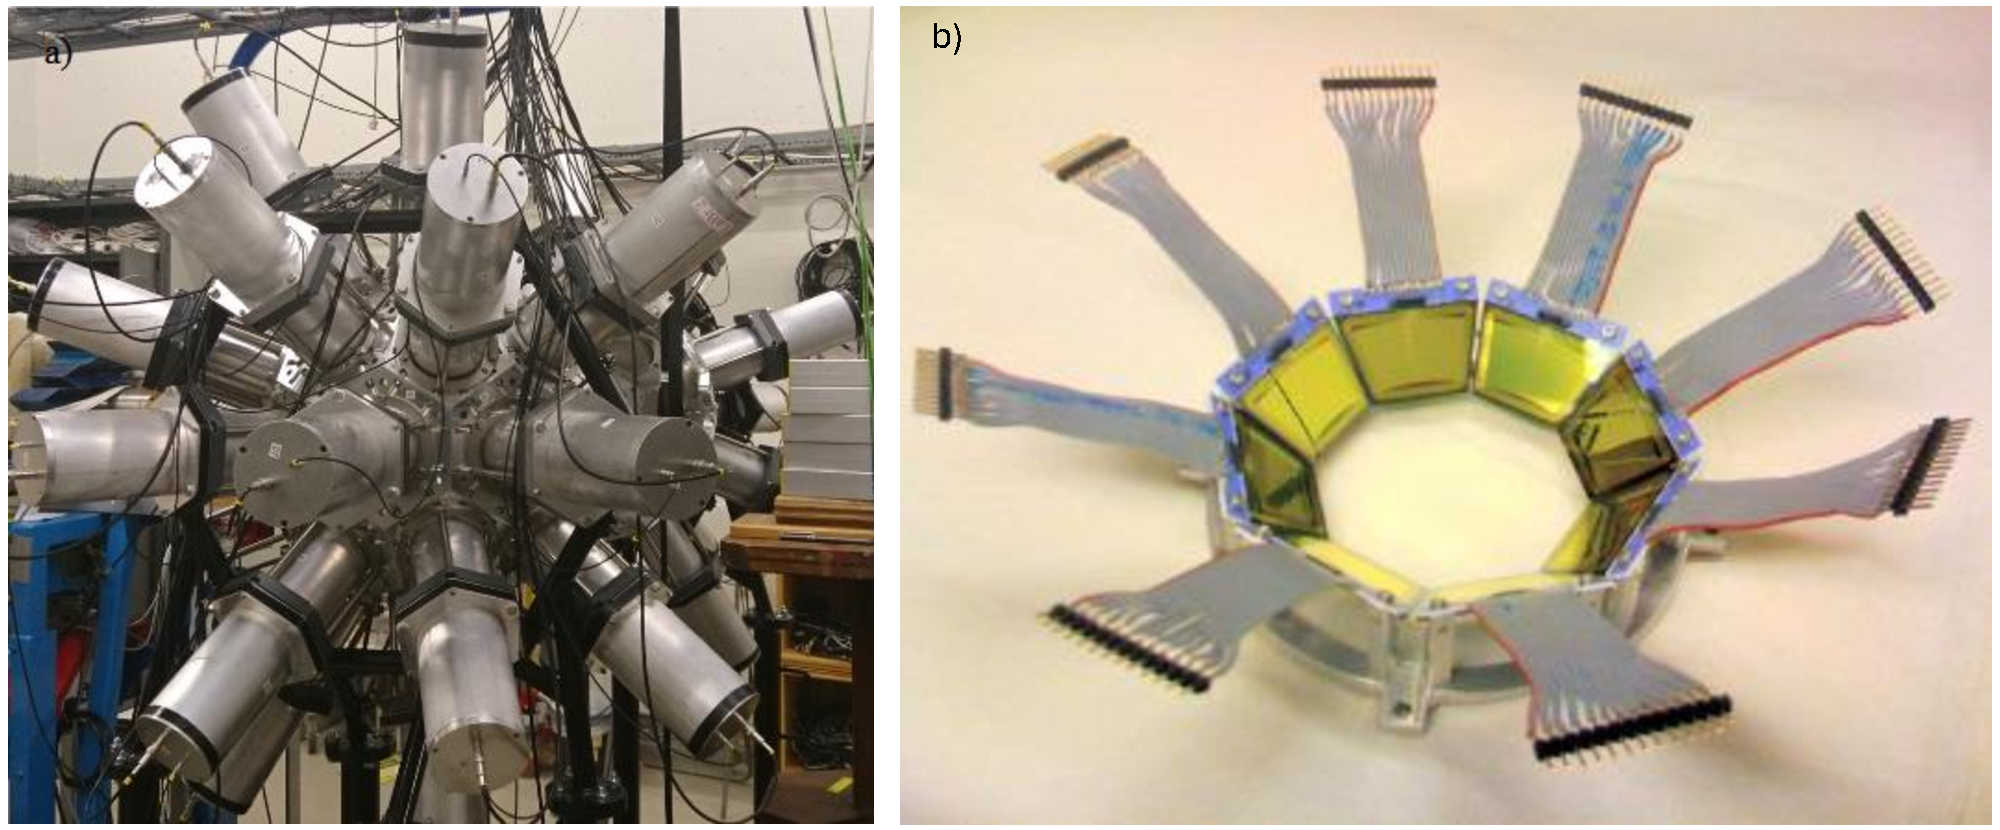
\includegraphics[width=0.8\linewidth]{figures/SiRi_OSCAR.pdf}
    \caption{Silicon ring detector (SiRi)\cite{GUTTORMSEN2011168} and The solid scintillation detector array OSCAR at the Oslo Cyclotron Laboratory\cite{MMarkova}}
    \label{fig:SiRi-OSCAR}
\end{figure}



\subsubsection{Bethe-Block formula} \label{subsubsec:bethe-block}
The relation between $E$ and $\Delta E$ can determine the type of particle by the relation $-\frac{dE}{dx} \propto z^2M/E$. The heavier a particle is, the more energy it will offset per distance in the detector material, which gives clear separation between particles of different masses and charges. 
\begin{equation}
    -\frac{dE}{dx} = 2\pi N_a r_e^2 m_e c^2 \rho \frac{Z}{A} \frac{z^2}{\beta^2} \left[ \ln\left(\frac{2m_e \gamma^2 v^2 W_{\max}}{I^2}\right) - 2\beta^2 - \delta - 2\frac{C}{Z} \right]
\end{equation}
where the constants and variables are defined as\cite{LEO}:
\begin{align*}
&A - \text{atomic weight of absorber} & &\rho - \text{density of absorber} \\
&Z - \text{atomic number of absorber} & &z - \text{charge of an incident particle} \\
&N_a - \text{Avogadro's constant} & &\beta - v/c \\
&m_e - \text{electron mass} & &\gamma - \text{Lorentz factor } 1/\sqrt{1 - \beta^2} \\
&r_e - \text{classical electron radius} & &\delta - \text{density correction} \\
&I - \text{mean excitation potential} & &C - \text{shell correction} \\
&W_{max} - \text{maximum energy transfer per collision}
\end{align*}

\subsubsection{Kinematics calculations with the \textsc{Qkinz} code}
The \textsc{Qkinz} software package was used to estimate energies deposited in the $E$ and $\Delta E$ detectors based on theoretically predicted values\cite{MMarkova,qkinz}. Included in the calculation parameters were thickness of target, angle of detector, intensity of the beam and assumed dead layer thickness. The software calculates energies of the excited states of projectiles from reaction pathways emitting charged particles denoted as $E_\text{calculated}$ and $\Delta E_\text{calculated}$. Coefficients to calculate excitation for calibrated $E = E+\Delta E$ are also given. 

\subsubsection{Excitation energies}
Converting $E_\text{sum} = E + \Delta E$ to excitation energies is done using the \textsc{Qkinz} calculated shift $b_0$, gain $b_1,$ and second order correction $b_2$ as in 
\begin{equation}
    E_\text{ex} = b_0 +  E_\text{sum}\cdot b_1 +  E_\text{sum}^2 \cdot b_2 
\end{equation}

\subsection{Photon energy detector array - OSCAR}
OSCAR is a solid scintillator detector array consisting of 30 LaBr$_3$ detectors mounted in a icosahedron-shaped frame. The working principle of a scintillator detector is to excite and de-excite the electrons of the crystal atoms to create cascades of visible light proportional to the energy of the incident photon. The visible photons in turn interact with the PM-tube, creating an electric pulse for the signal processing systems to utilize. 
LaBr$_3$ detectors have good resolution at $\approx2.7-4.3\%$ at 662 keV, with relatively high counting rate due good light output ($\approx63000$ photons/MeV)\cite{MMarkova}. One can determine the full width at half maximum (FWHM) and thereby the resolution by \cref{eq:resolution}. If peaks are one or more FWHMs apart, they are regarded as separately resolved. 

\begin{equation}
\mathrm{FWHM} =2\sqrt{2ln2}\,\sigma, 
\qquad 
R(E) \equiv \frac{\mathrm{FWHM}}{E}
\label{eq:resolution}
\end{equation}



\subsection{Calibration and signal processing}
\subsubsection{ROOT}
ROOT is a program used to analyze large amounts of data, most typically within some genre of particle physics. Data processing in this project is done through pre-prepared programs written in ROOT C++, with modifications when needed. Visualization is also done with ROOT.


\subsubsection{Electronics and data acquisition}
Handling of the electronics and the data acquisition processes were not part of the scope of this project. 

\newpage
\section{Method}
\subsection{Data acquisition}
In this report there are three runs. Two of them are for the \nuclide[106]{Pd}$(p,p'\gamma)$\nuclide[106]{Pd} data collection, while the \nuclide[27]{Al} run is for calibration. 


The detectors are  connected to Digital Gamma Finders (DFG), which combine spectroscopy with digitizing and pulse-shape analysis, also support coincidence measurements. For OSCAR, each of the DFGs sample with 250 MSPS(MHz) frequency. SiRi on the other hand has a sampling frequency of 250 MSPS for $\Delta E$ and 500 MSPS for the $E$-detector \cite{MMarkova}. 

\subsection{SiRi calibration}

The calibration of SiRi occurs post experiment and can be broken into two main processes. The first sorting is a rough sorting, while the second is a finer sorting where energies are applied to measurements. The data-processing iterative method is outlined in \cref{fig:flowchart}. With \nuclide[106]{Pd} being heavy so recoil energy can be disregarded, while also being the nuclide of interest, it is chosen for SiRi calibration. 

\subsubsection{Rough sorting}

A wide time gate of 2000 ns is applied for $E -\Delta E$ coincidences, with plain calibration coefficients. The data is converted from .data to .root-format. Bad detector combinations are identified and removed. The result is an uncalibrated $E\Delta E$, e.g \cref{fig:EdE-uncalibrated-106Pd}. The bad detector combinations were identified to be: all combinations including back-detector 2, as well as b1f7, b3f7, b5f6, b5f7 and b7f7.
\begin{figure}
    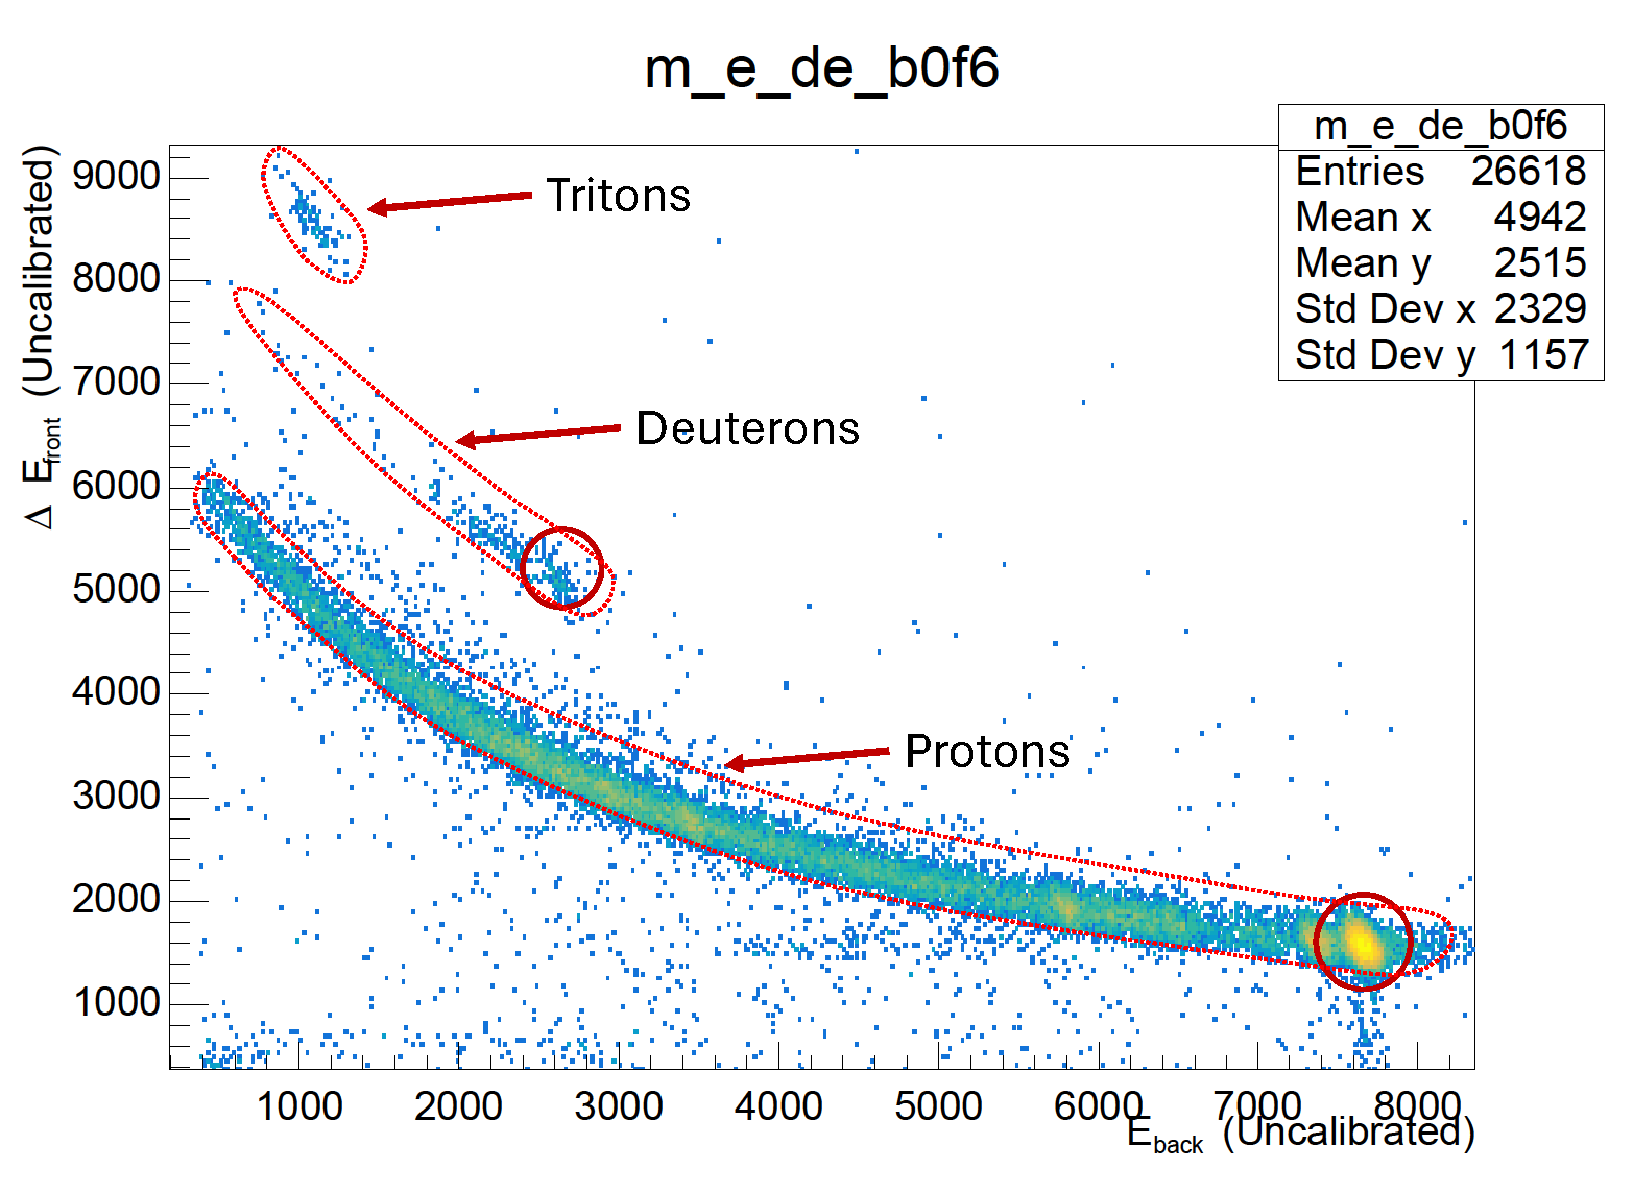
\includegraphics[width=0.6\linewidth]{figures/FYS2810-SiRi-uncalibrated.pdf}
    \centering
    \caption{Uncalibrated $E\Delta E$ plot of detector combination b0f6 for \nuclide[106]{Pd}. Protons, deuterons and tritons can be observed by their corresponding bananas. The points marked with red circles are used for calibration, as they represent the highest energy a particle can offset in the detector following the lowest excited level of a nucleus. The clear separation of particles is explained by the Bethe-Block formula (\cref{subsubsec:bethe-block}).}
    \label{fig:EdE-uncalibrated-106Pd}
\end{figure}

\subsubsection{Fine sorting}
The 0 keV exitation peaks for the protons and deutrons are identified as in \cref{fig:EdE-uncalibrated-106Pd} for all 64 detector combinations, determining $E_\text{measured}$ and $\Delta E_\text{measured}$. Calibration coefficients for linear calibration are determined using \cref{eq:a1b1} and \cref{tab:Qkinz-ground-state}. Actual energies are determined using \cref{eq:linear-fit}, and spectra are re-calibrated with coefficients accordingly. An energy cut limiting the energies to those contained within the proton banana is set, similar to \cref{fig:EdE-uncalibrated-106Pd}. The contained energies are converted to excitation energies using \textsc{Qkinz} excitation coefficients (\cref{tab:Qkinz-excitation-values}). Each ring is shift adjusted to align first excitation peak at 0 keV. Calibrated peaks are compared to known values to assure correct calibration. 

\begin{table}[htbp]
    \centering
    \caption{Qkinz values for deposited energy for the ground state energies of the protons from \nuclide[106]{Pd}$(p,p'\gamma)$\nuclide[106]{Pd} and deuterons from \nuclide[106]{Pd}$(p,d\gamma)$\nuclide[105]{Pd} (left), and \textsc{Qkinz} excitation coefficients for \nuclide[106]{Pd} (right).}
    \begin{minipage}{0.55\textwidth}
        \centering
        \begin{tabular}{c S[table-format=6.2] S[table-format=4.2] | S[table-format=4.2] S[table-format=4.2]}
            \toprule
            & \multicolumn{2}{c|}{Proton} & \multicolumn{2}{c}{Deuteron} \\
            \cmidrule(r){2-3} \cmidrule(l){4-5}
            {Strip} & {$E$ (keV)} & {$\Delta E$ (keV)} & {$E$ (keV)} & {$\Delta E$ (keV)} \\
            \midrule
            $f_0$ & 14648.95 & 798.55  & 5689.54 & 2388.91 \\
            $f_1$ & 14658.65 & 795.29  & 5707.27 & 2377.23 \\
            $f_2$ & 14667.60 & 793.04  & 5721.86 & 2368.88 \\
            $f_3$ & 14675.78 & 791.77  & 5733.33 & 2363.81 \\
            $f_4$ & 14683.19 & 791.47  & 5741.70 & 2362.00 \\
            $f_5$ & 14689.82 & 792.16  & 5746.93 & 2363.44 \\
            $f_6$ & 14695.64 & 793.82  & 5748.99 & 2368.15 \\
            $f_7$ & 14700.62 & 796.49  & 5747.78 & 2376.18 \\
            \bottomrule
        \end{tabular}
        \label{tab:Qkinz-ground-state}
    \end{minipage}%
    \hfill\hfill
    \begin{minipage}{0.40\textwidth}
        \centering
        \begin{tabular}{cc|c|c}
            \toprule
            Strip & $b_0$ (keV) & $b_1$  & $b_2$ (1/keV) \\
            \midrule
            $f_0$ & $15.735\cdot 10^{3}$ & $-1.020702$ & $0.000137\cdot 10^{-3}$ \\
            $f_1$ & $15.735\cdot 10^{3}$ & $-1.020136$ & $0.000125\cdot 10^{-3}$ \\
            $f_2$ & $15.740\cdot 10^{3}$ & $-1.019541$ & $0.000113\cdot 10^{-3}$ \\
            $f_3$ & $15.736\cdot 10^{3}$ & $-1.018912$ & $0.000099\cdot 10^{-3}$ \\
            $f_4$ & $15.737\cdot 10^{3}$ & $-1.018252$ & $0.000085\cdot 10^{-3}$ \\
            $f_5$ & $15.737\cdot 10^{3}$ & $-1.017559$ & $0.000069\cdot 10^{-3}$ \\
            $f_6$ & $15.737\cdot 10^{3}$ & $-1.016830$ & $0.000053\cdot 10^{-3}$ \\
            $f_7$ & $15.737\cdot 10^{3}$ & $-1.016073$ & $0.000037\cdot 10^{-3}$ \\
            \bottomrule
        \end{tabular}
        \label{tab:Qkinz-excitation-values}
    \end{minipage}
\end{table}




\begin{figure}
    \centering
    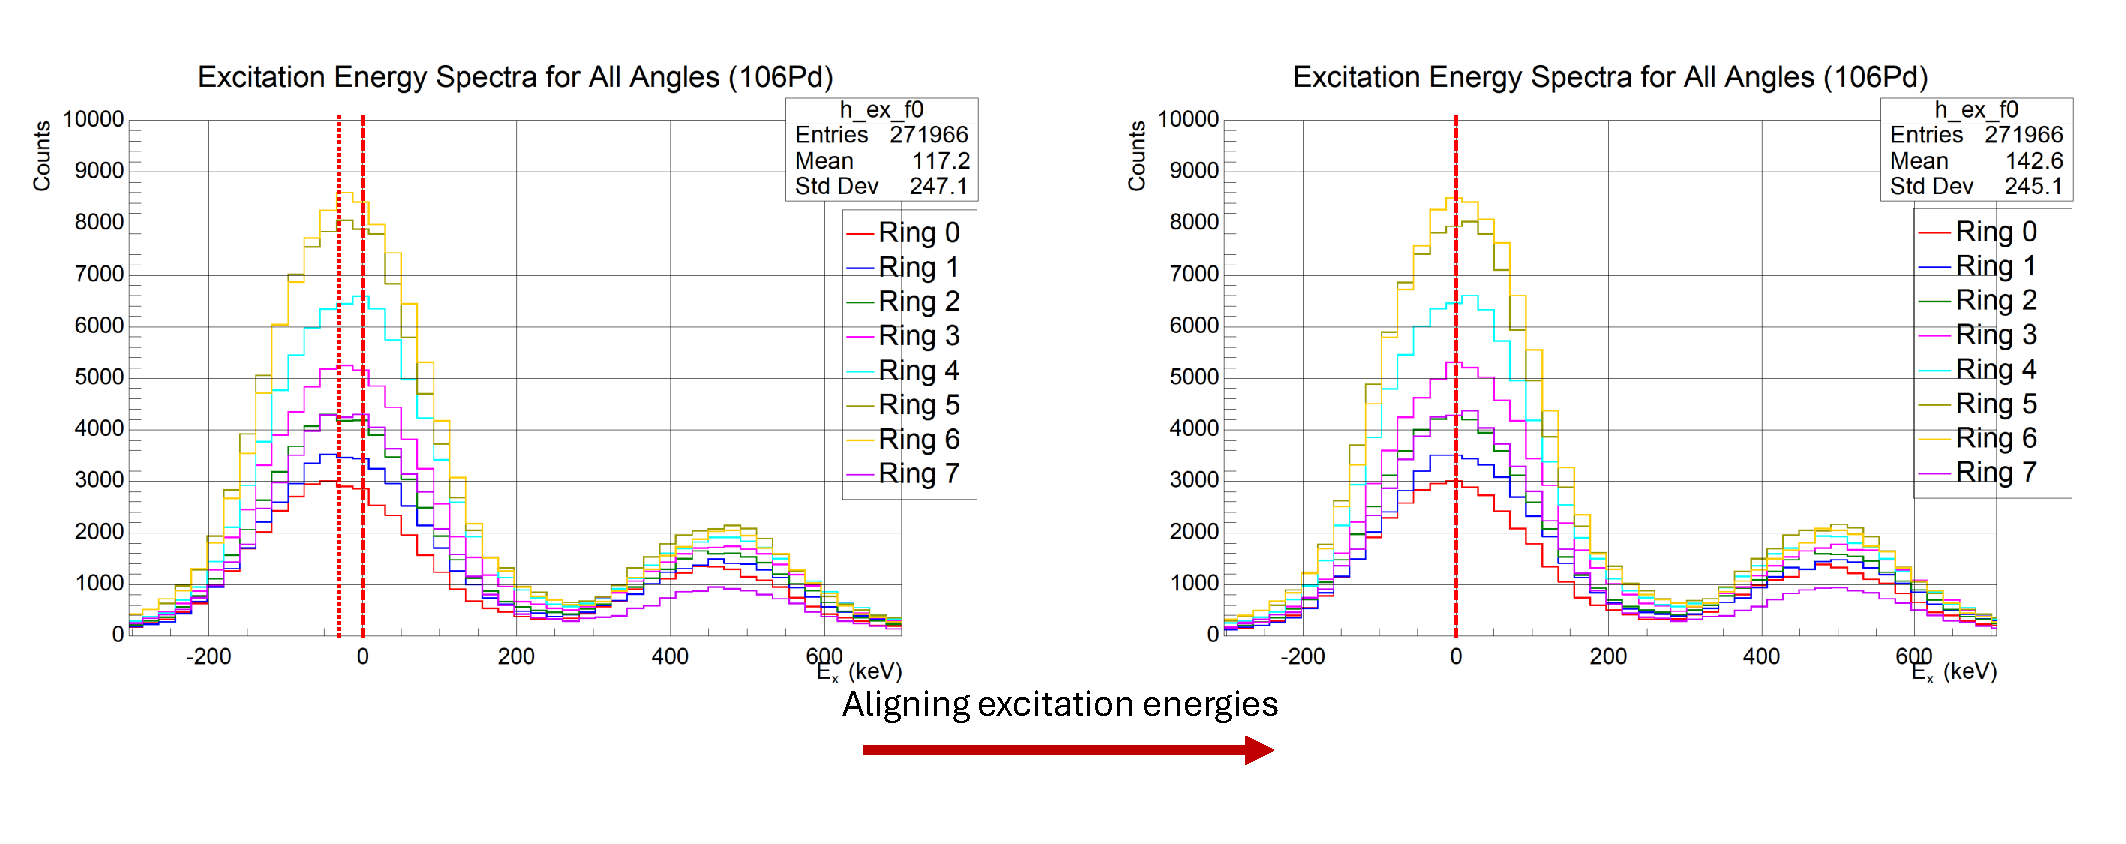
\includegraphics[width=\linewidth]{figures/106Pd-excitation-energies.pdf}
    \caption{After the initial calibration, a shift was added to the excitation energies so that the first excitation centroids for all rings f0-f7 align with 0 keV}
    \label{fig:excitation-shift}
\end{figure}


% \nuclide[106]{Pd} - little recoil since large :)\\





\subsection{OSCAR calibration}
For calibration of the solid scintillator array OSCAR, the known calibration isotope \nuclide[27]{Al} was chosen. Using the energy peaks of 511 keV and 3004.2 keV for the calibration covers the most important range of $\gamma$-decay energies for \nuclide[106]{Pd}. If calibration of \nuclide[27]{Al} is done well, applying said calibration to \nuclide[106]{Pd} will reproduce known $E_\gamma$ values.



All bad detectors with unreasonably large FWHMs are removed. The 551 keV and 3004.2 keV energy peaks are identified on each detector. Calibration coefficients $a_0$ and $a_1$ are determined using the least squares method in Excel called LINEST for each detector. A linear calibration as in \cref{eq:linear-fit} is applied. A time and energy gate for OSCAR-SiRi coincidences is set. If OSCAR detects in a time window of 220 to 270 ns (\cref{fig:106Pd-timegate}) after SiRi and it is within the proton cut energies of SiRi, the excitation matrix and $\gamma$-energy spectra is filled with said energies. Similarly the background matrix was also filled, but with a time window of 330 to 390 ns. When approproate, resolutions of energy peaks are calculated using \cref{eq:resolution}. With OSCAR-SiRi coincidences registered, the Excitation vs. Gamma energy matrix can be constructed. 

\begin{figure}
    \centering
    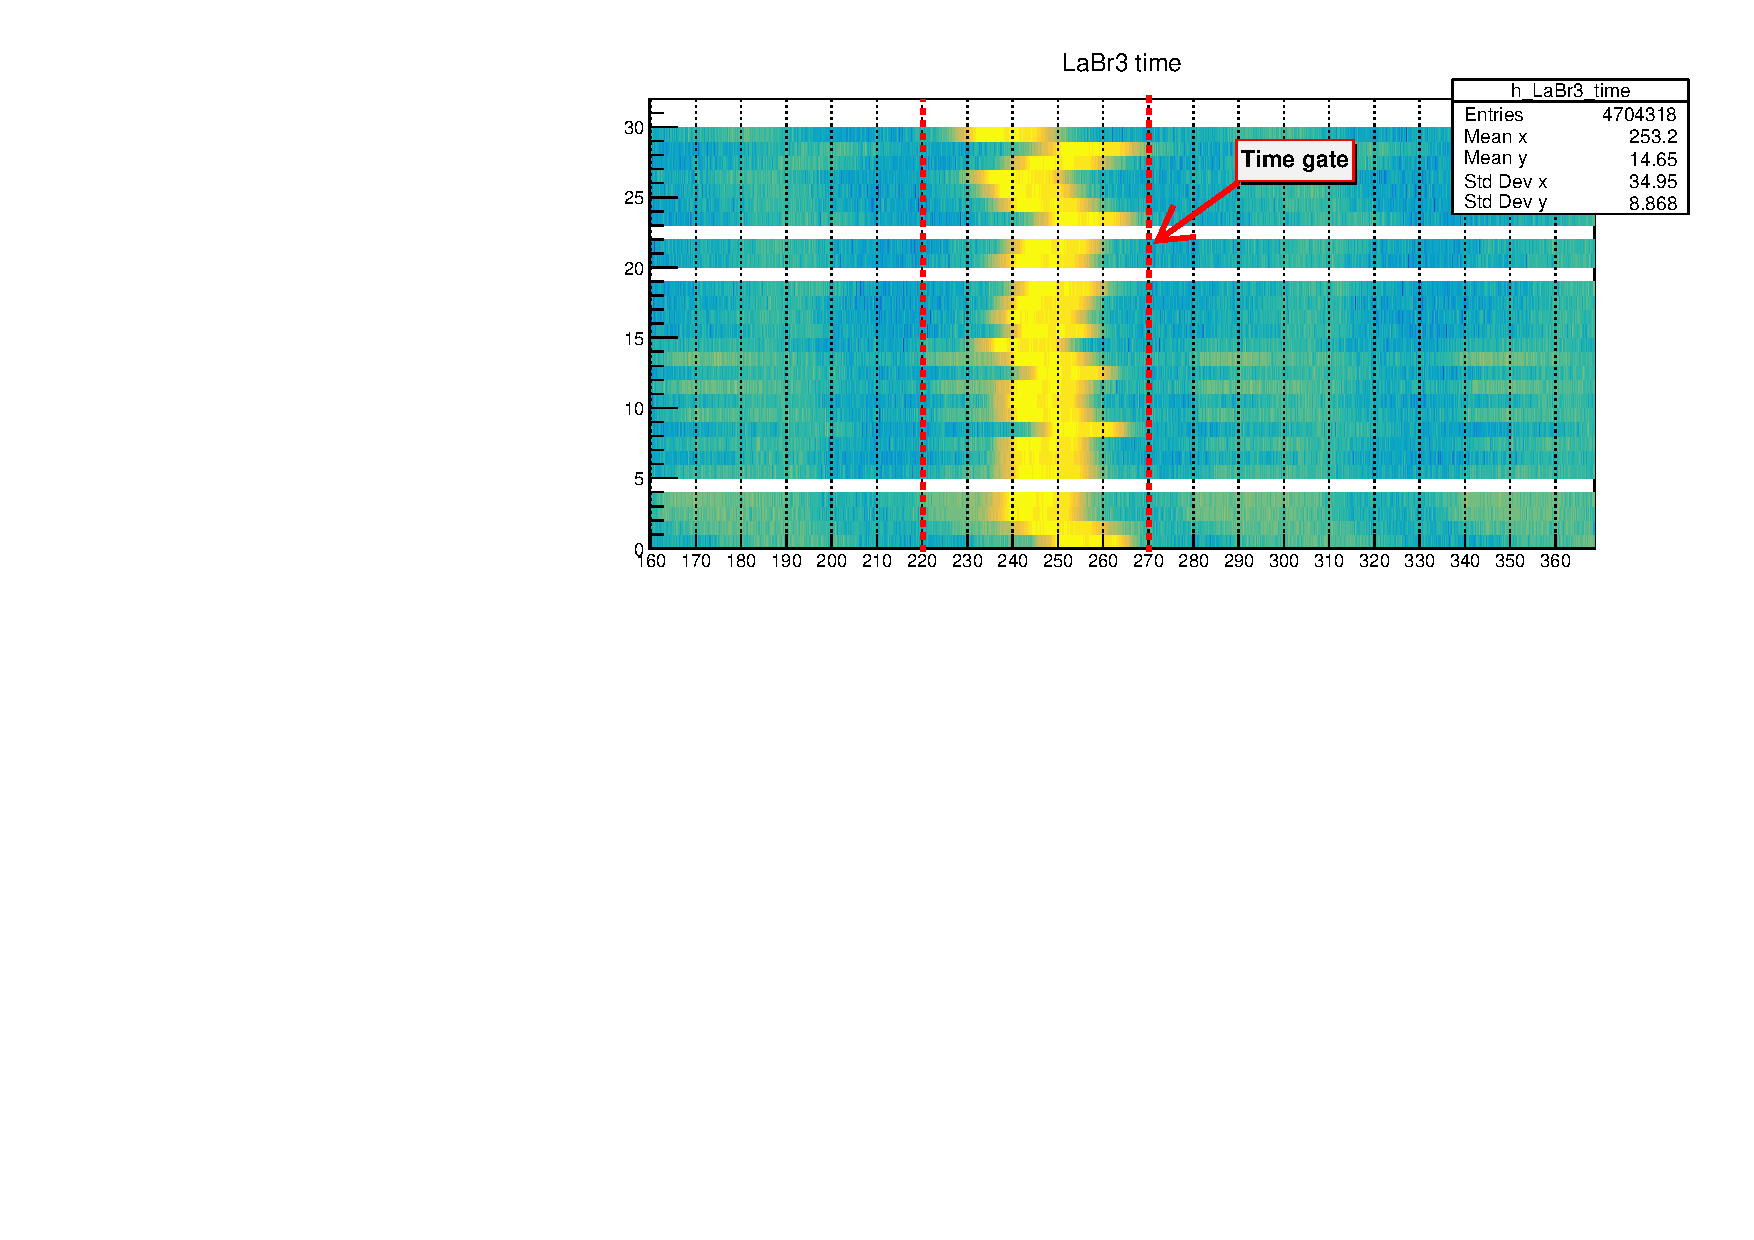
\includegraphics[width=0.75\linewidth]{figures/106Pd_27th_timegate.pdf}
    \caption{The time gate of 220 to 270 ns applied for acquiring OSCAR-SiRi coincidences is shown. It is seen that the pulse of interest is contained within the time gate.}
    \label{fig:106Pd-timegate}
\end{figure}


\newpage
\section{Results}
% \begin{itemize}
%     \item \nuclide[27]{Al} spectra - quality of calibration
%     \item \nuclide[106]{Pd} spectra
%     \item Excitation spectra
%     \item EdE spectra
%     \item Excitation matrix
%     \item time (discussion?)
%     \item Resolution
% \end{itemize}
\subsection{OSCAR calibration}


% \subsubsection{\nuclide[27]{Al} $\gamma$-energy spectra}
The calibration of \nuclide[27]{Al} mostly reproduce known database values (\cite{27Al}). The $\gamma$-energy spectra for \nuclide[27]{Al} are shown in \cref{fig:27Al-combined,fig:27Al-det1}, for all detectors combined and detector 1 alone. Fits (\cref{tab:27Al-combined-fits}) done on the calibration peaks of 511 and 3004.2 are in good agreement with database values for the combined fit, but deviates about 7 keV for the peak of 2212 keV which was not calibrated for. The fits to detector 1 fare similarly, but show a deviation for both 2212 keV and 3004 keV of up to 5 keV. 

\begin{figure}[htbp]
    \centering
    \begin{minipage}{1\textwidth}
        \centering
        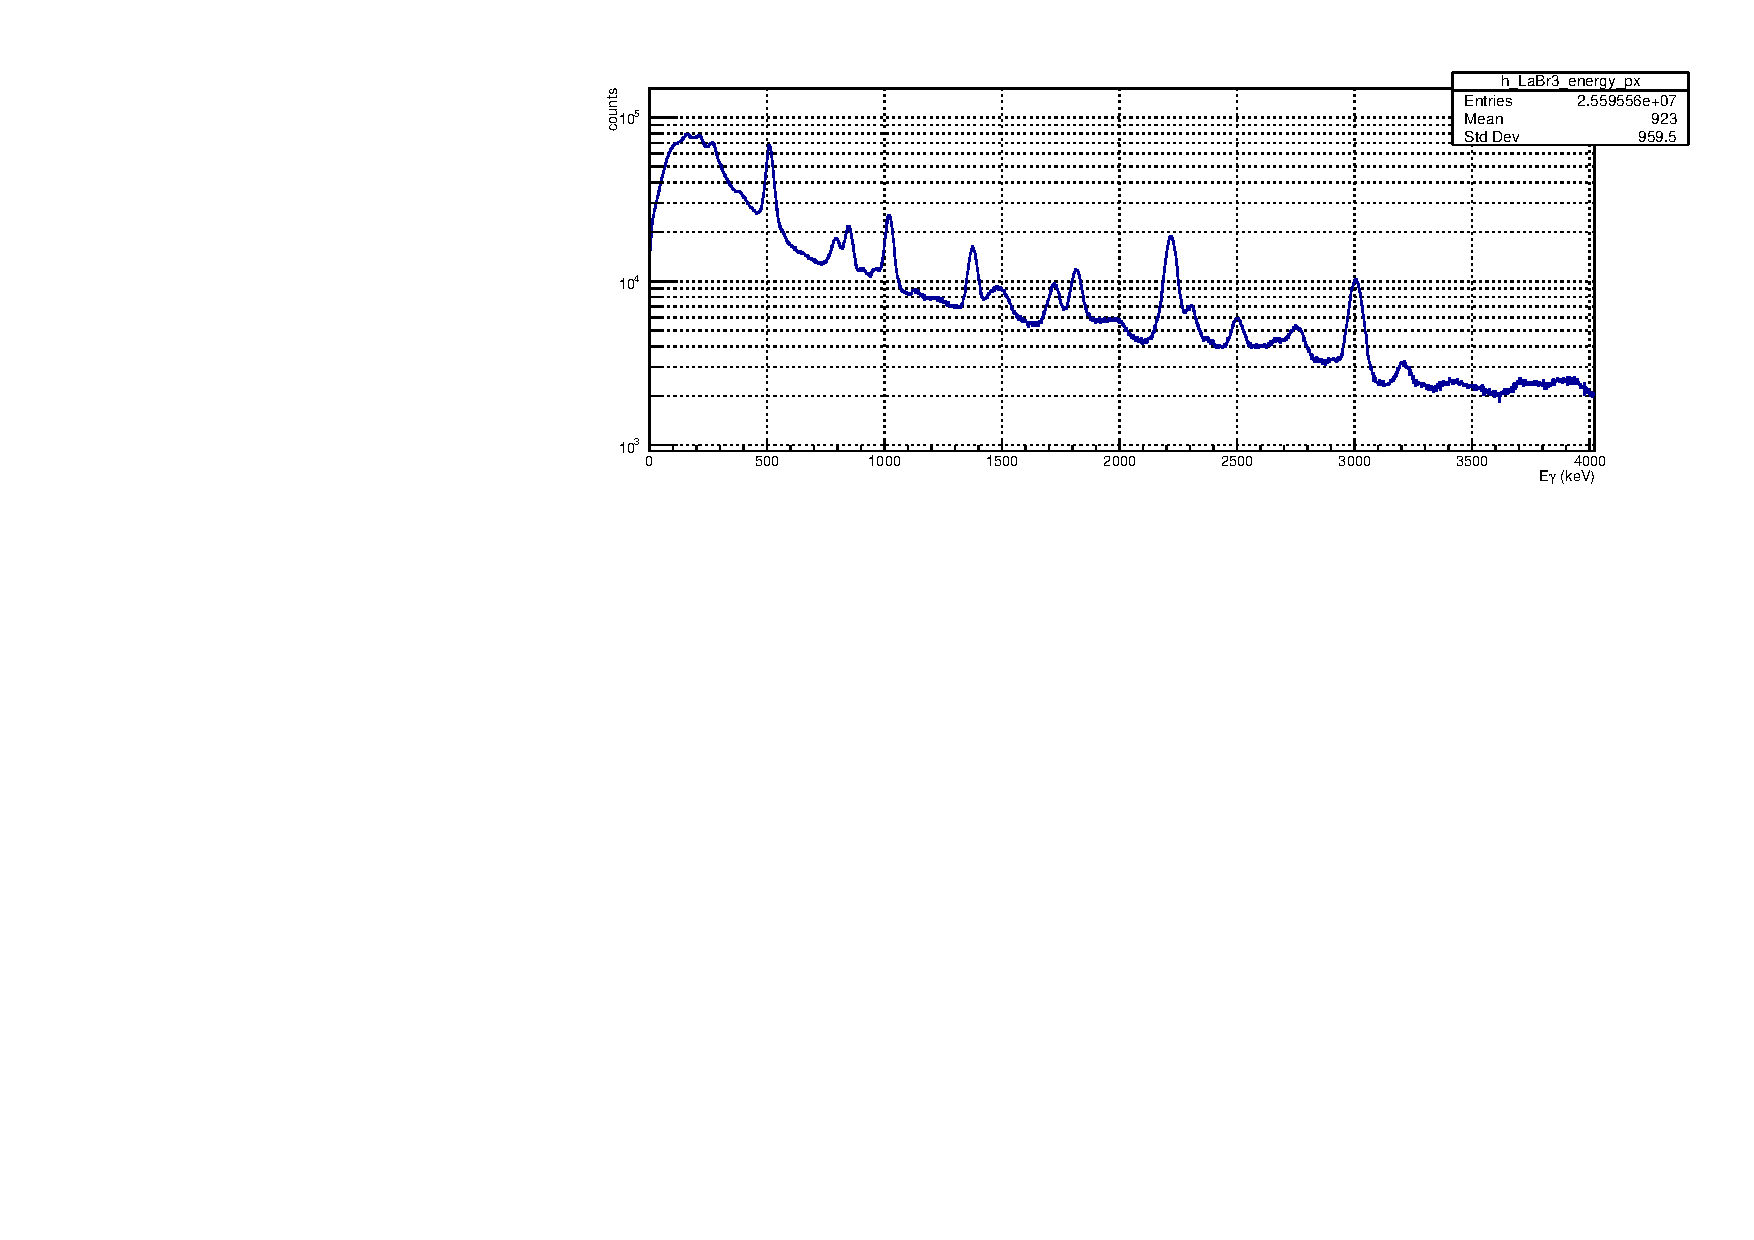
\includegraphics[width=\textwidth]{figures/27Al_gamma_combined.pdf}
        \caption{Combined \nuclide[27]{Al} $\gamma$-energy spectra with peaks 511 keV, 2212.01 keV and 3004.2 keV fits described in \cref{tab:27Al-combined-fits}. Each bin represents 2 keV each.}
        \label{fig:27Al-combined}
    \end{minipage}
    \hfill
    \begin{minipage}{1\textwidth}
        \centering
        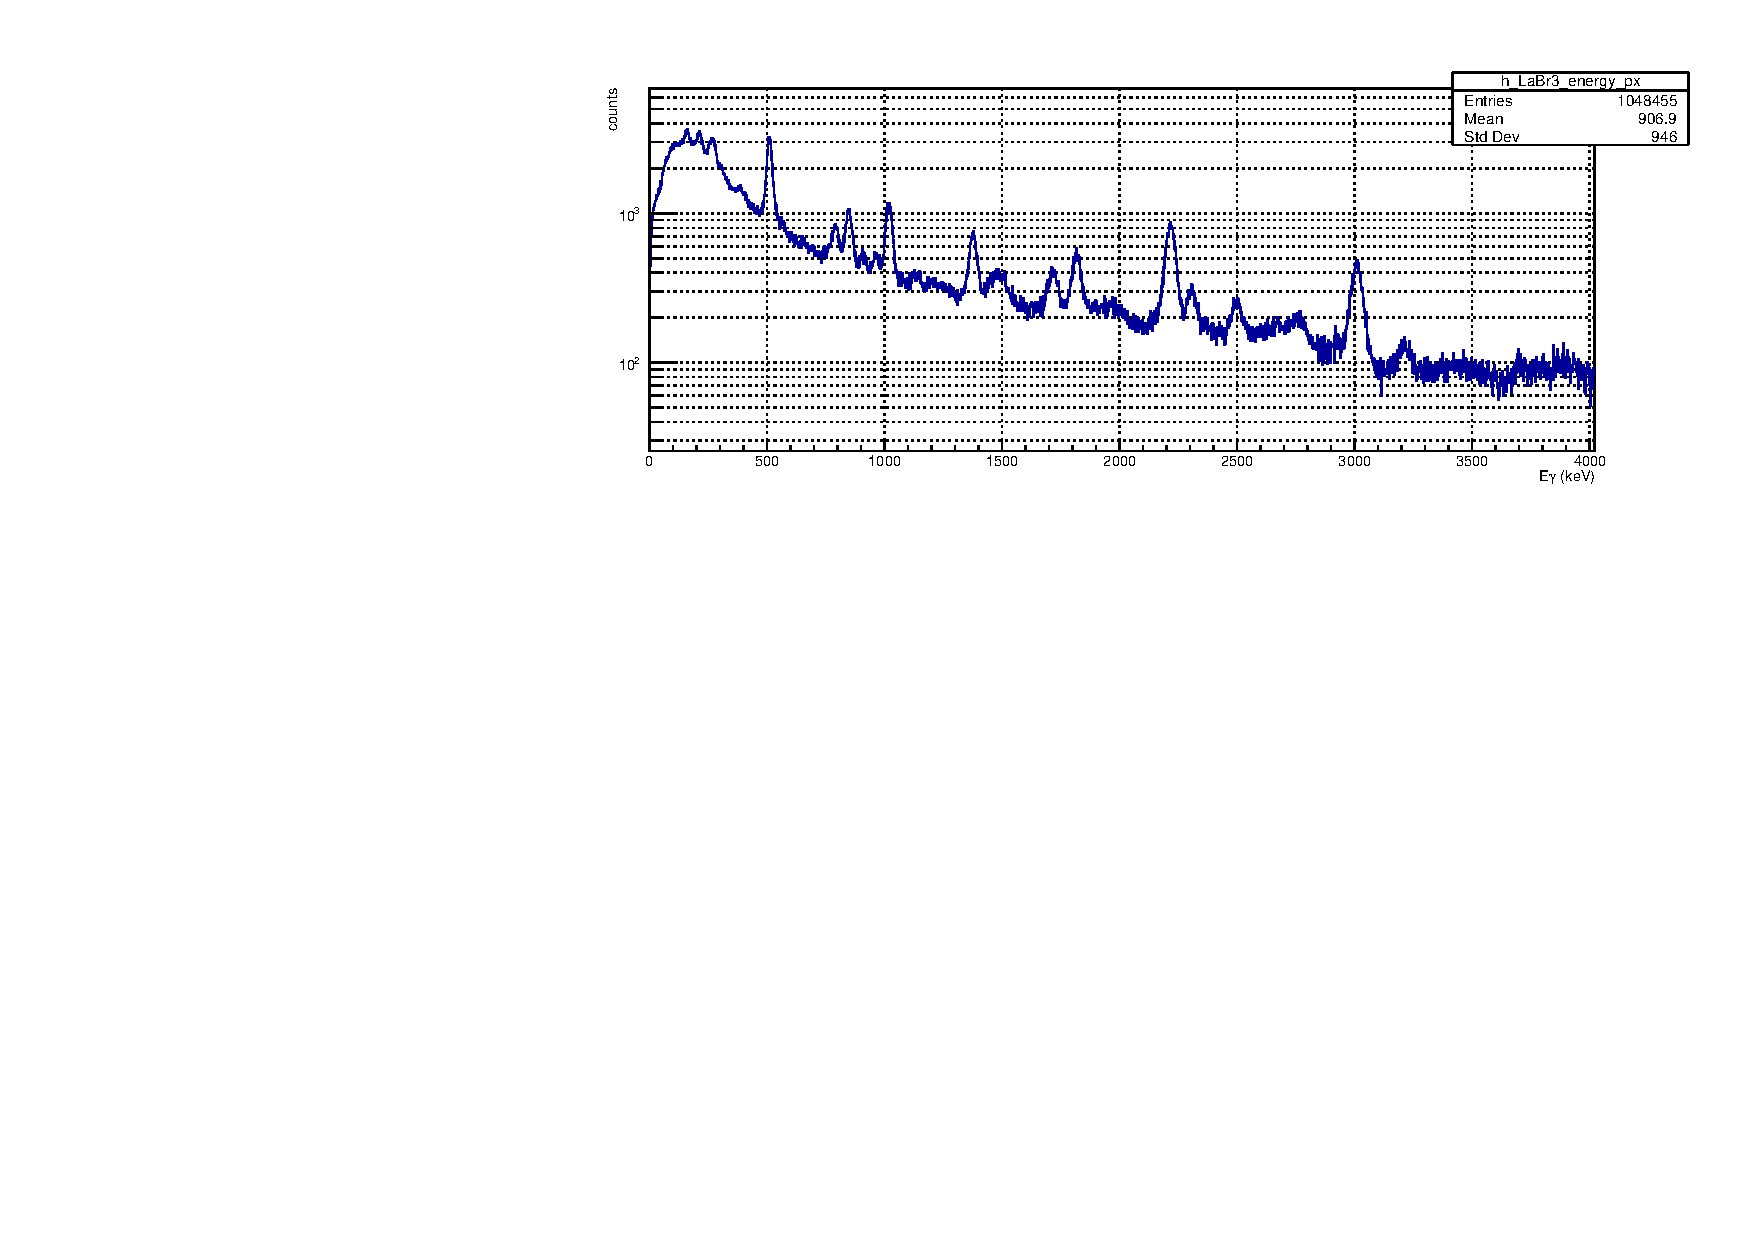
\includegraphics[width=\textwidth]{figures/27Al_gamma_det1.pdf}
        \caption{OSCAR detector 1 \nuclide[27]{Al} $\gamma$-energy spectra with peaks 511 keV, 2212.01 keV and 3004.2 keV fits described in \cref{tab:27Al-det1-fits}}
        \label{fig:27Al-det1}
    \end{minipage}
\end{figure}

% \subsubsection{\nuclide[106]{Pd} $\gamma$-energy spectra}

\begin{figure}
    \centering
    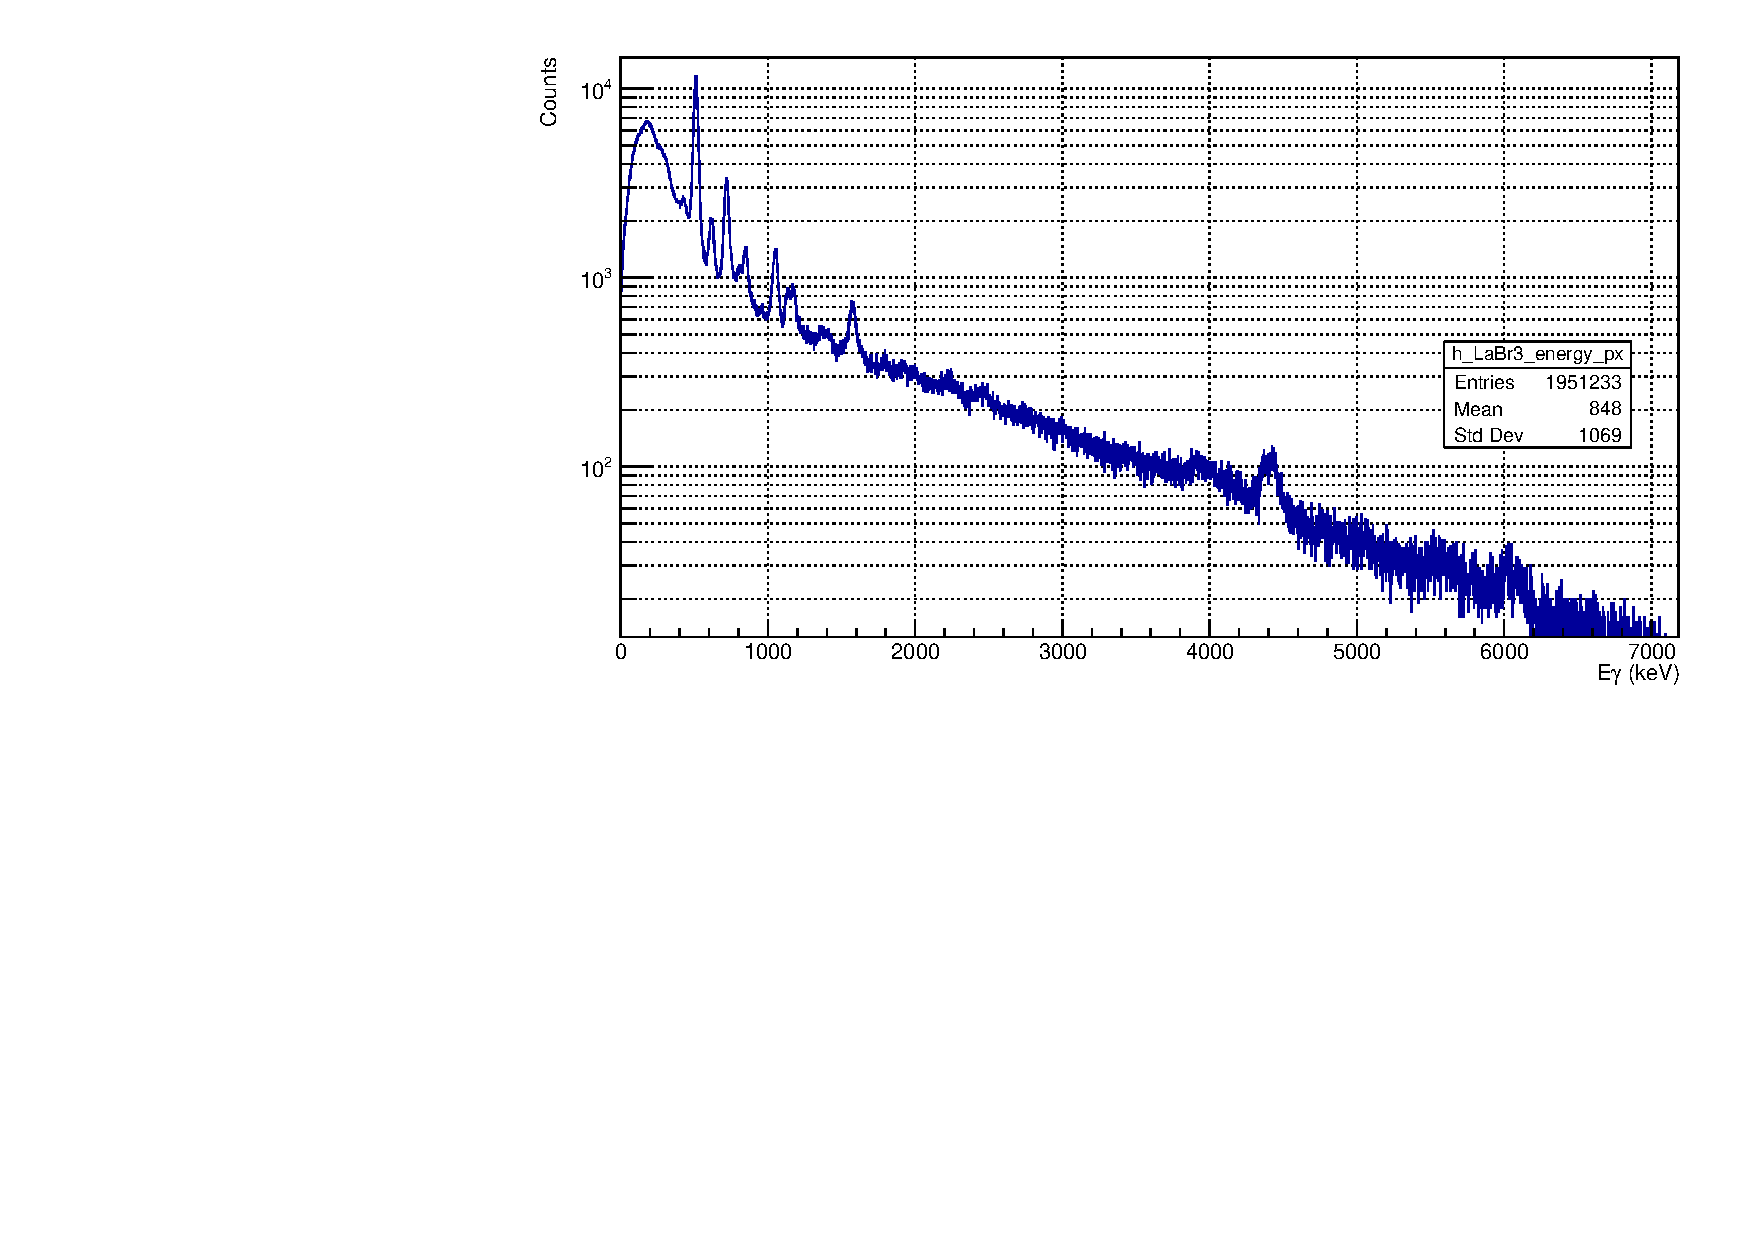
\includegraphics[width=0.8\linewidth]{figures/106Pd_27th_combined.pdf}
    \caption{The figure shows the resulting $\gamma$-energy spectra from the proton gated OSCAR-SiRi coincidences. Some peaks were fitted for with a simple gaussian to confirm calibration. The results are seen in \cref{tab:106Pd-fits}. The calibration both overshoots and undershoots by up to 5 keV in the calibration range of 0.5 to 3 MeV. Peaks at $\sim 4.4 $ MeV and $\sim 6$ MeV remain unknown, not observed in databases for \nuclide[104]{Pd}, \nuclide[105]{Pd} and \nuclide[106]{Pd}.}
    \label{fig:106Pd_Eg} 
\end{figure}
% The combined $E_\gamma$ calibrated plot for \nuclide[106]{Pd} (\cref{fig:106Pd_Eg}) seems to be in agreance to the database \cite{106Pd}. 


The calibrated \nuclide[106]{Pd} $\gamma$-energy spectra (\cref{fig:106Pd_Eg}) filled with SiRi-OSCAR coincidences with excitation energies correlating to \nuclide[106]{Pd}$(p,p'\gamma)$\nuclide[106]{Pd} agree mostly with database values \cite{104Pd,105Pd,106Pd}. Peaks up to 1572 keV were identified with fits within 5 keV of actual values (\cref{tab:106Pd-fits}). Peaks 1045 keV and 1050 keV are too close to each other and are unresolvable. Seen at $\sim 4.4$ MeV and $\sim 6$ MeV two unidentifiable peaks, not contained in databases for \nuclide[104]{Pd}, \nuclide[105]{Pd} and \nuclide[106]{Pd}. These both have large uncertainties to them because of low counts. 

\begin{figure}
    \begin{minipage}{0.45\textwidth}
        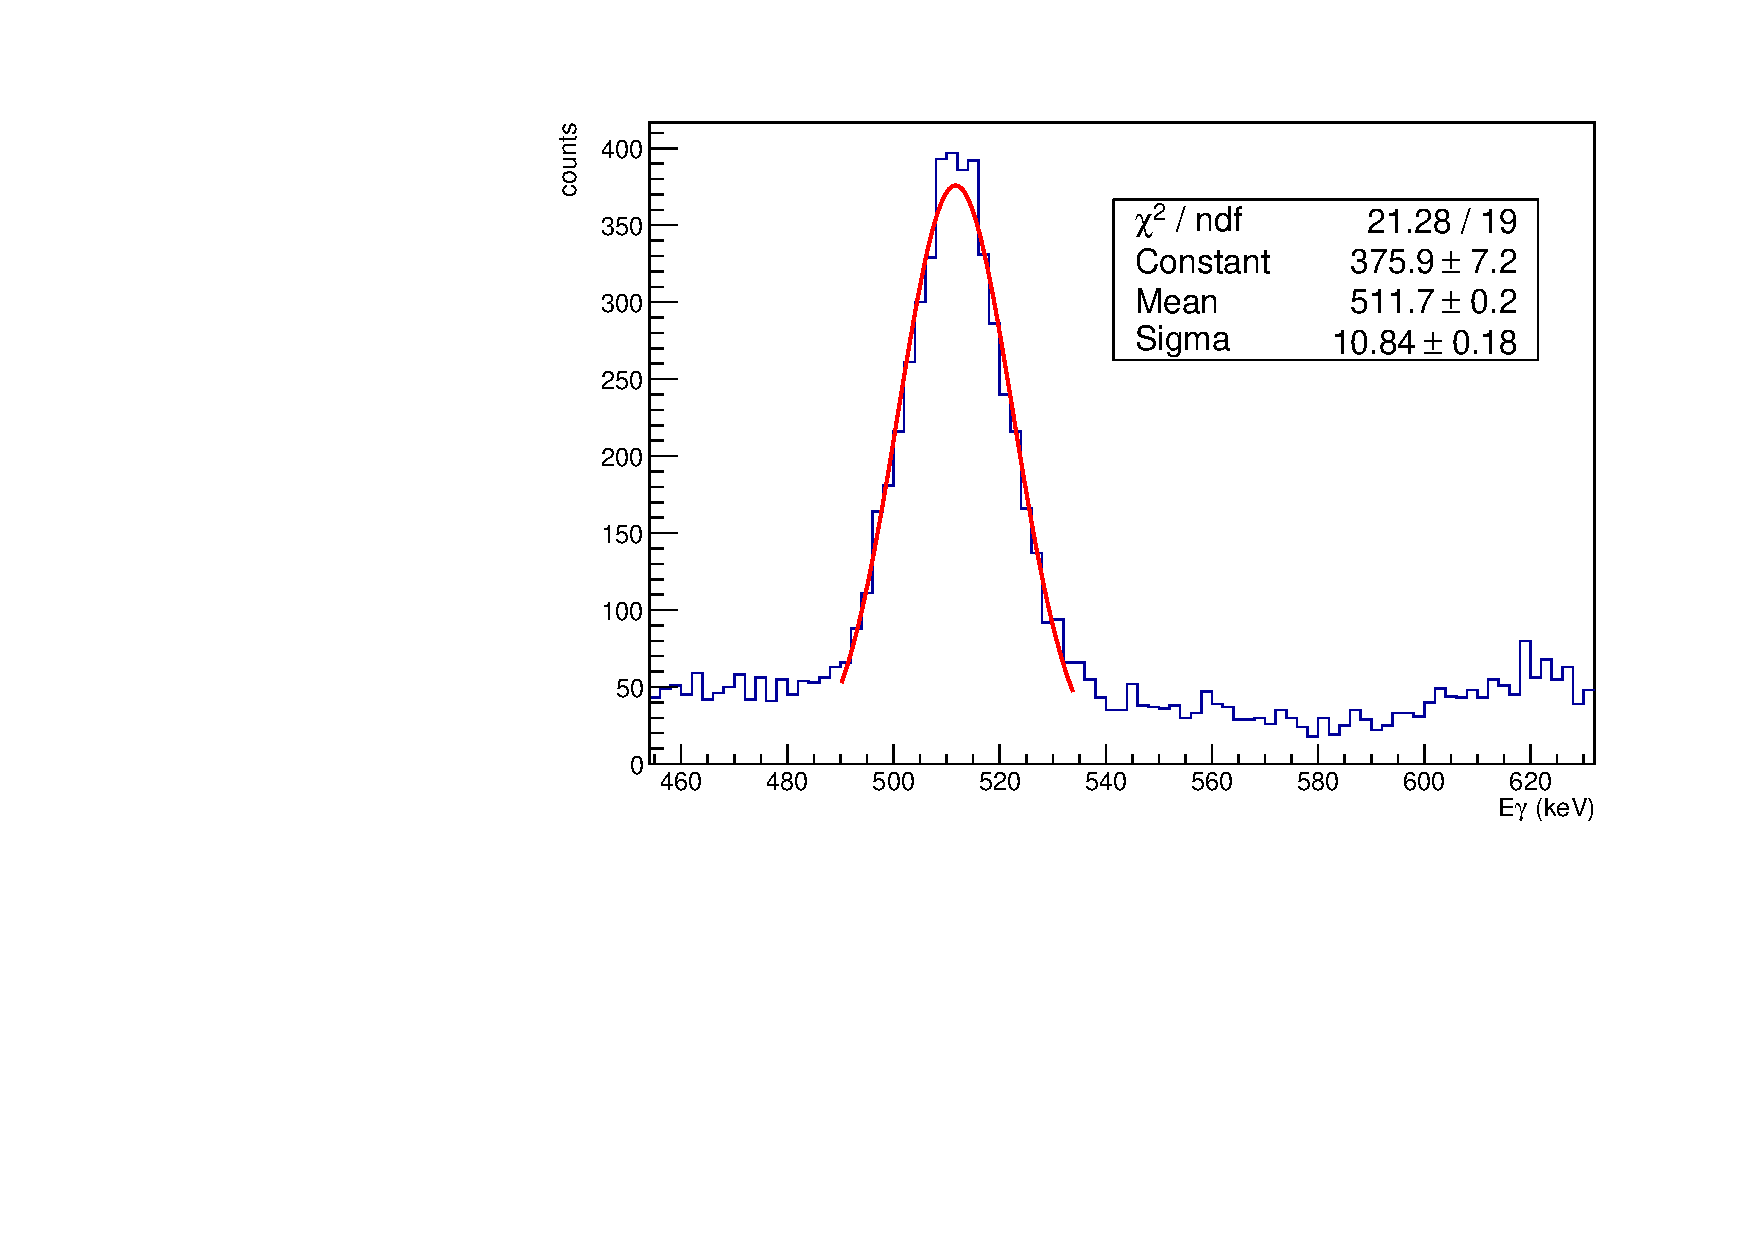
\includegraphics[width=1\linewidth]{figures/LaBr3_det1_106Pd.pdf}
    \end{minipage}
    \begin{minipage}{0.45\textwidth}
        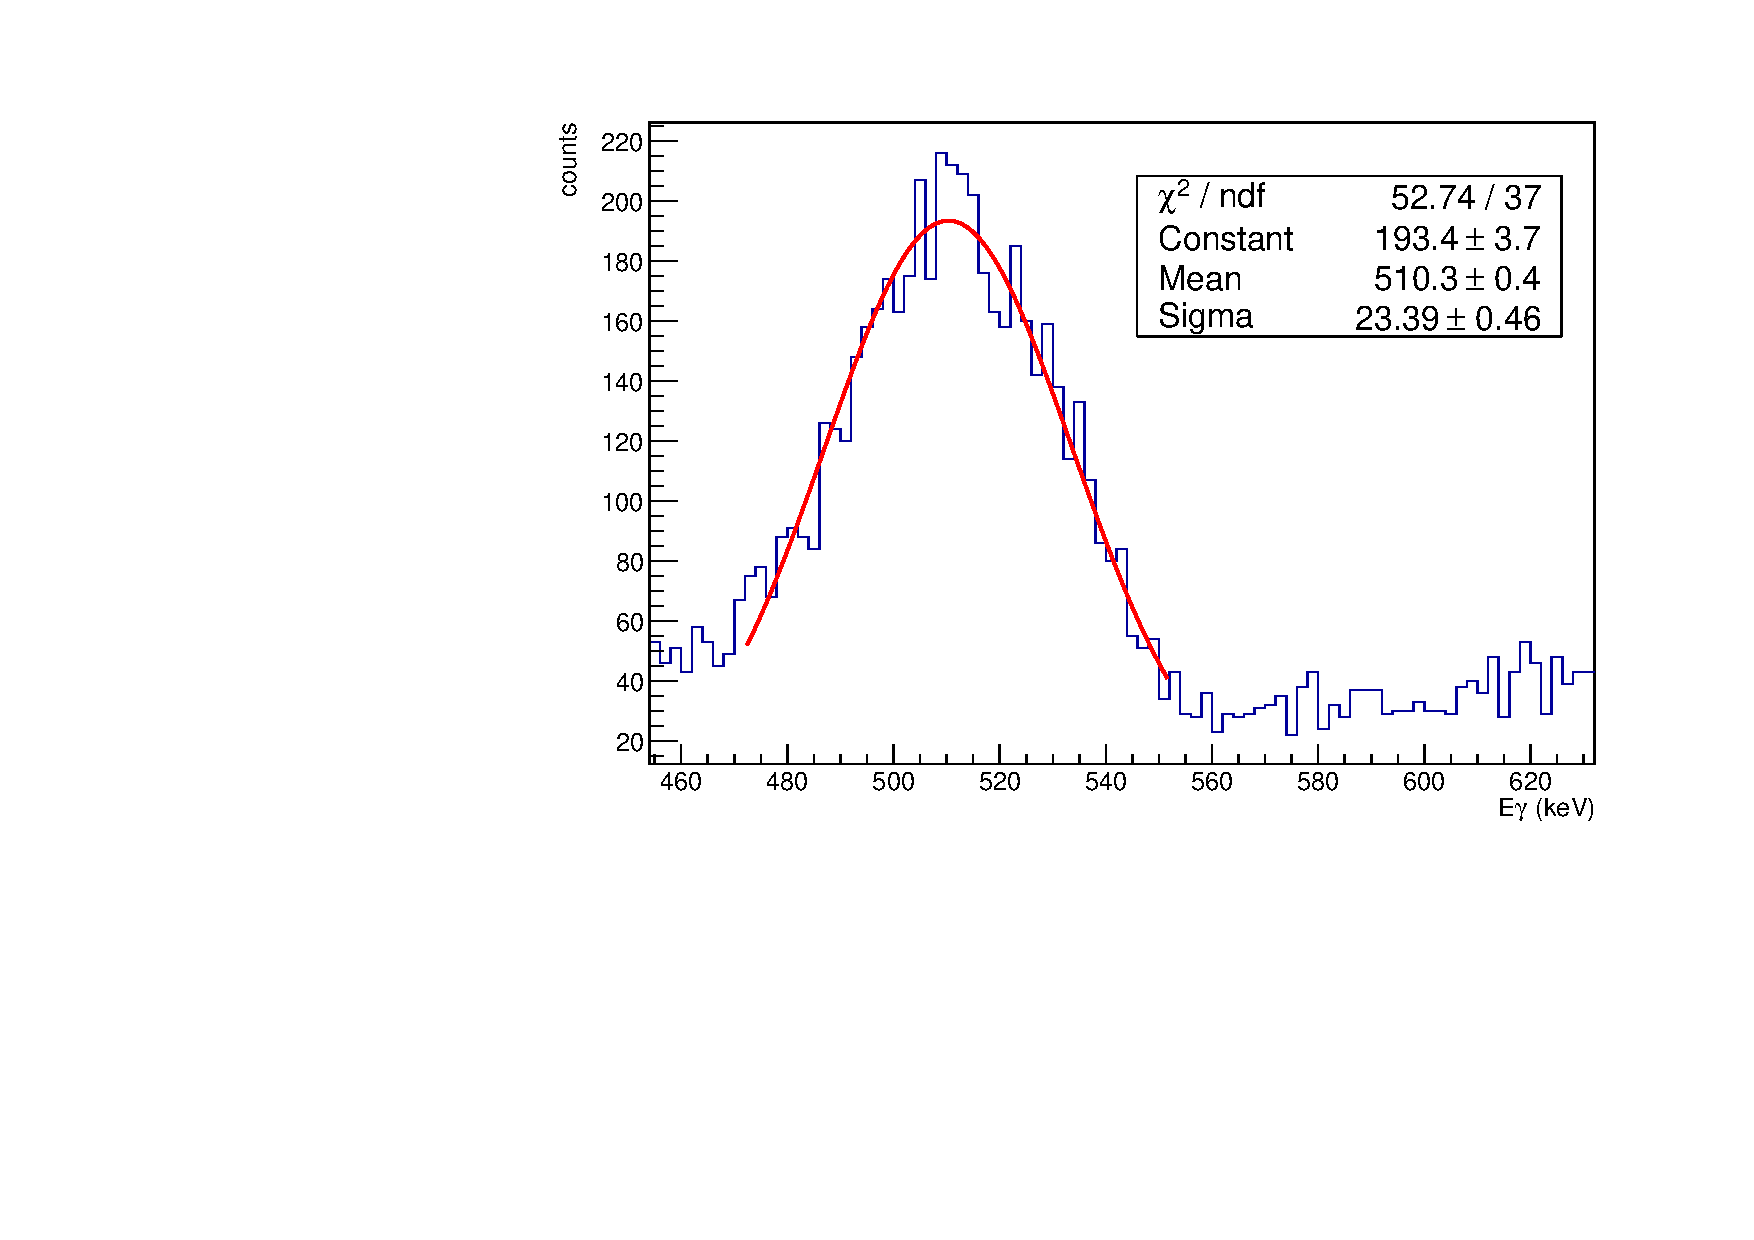
\includegraphics[width=1\linewidth]{figures/LaBr3_det6_106Pd.pdf}
    \end{minipage}
    \centering
    \caption{Figures showing resolution of the 511.850 keV peak for \nuclide[106]{Pd} \cite{106Pd}. Detector 1 had one of the best energy resolutions at $5.1\%$ compared to detector 6 with a resolution of $10.8\%$. Note that these are very rough fits where background hasn't been accounted for. The intent is to show the difference in resolution between detectors, which is clear. With several detectors with similar resolution to detector 6, the $\gamma$-energy spectra becomes smeared out, giving less accurate results.}
    \label{fig:106Pd-511.8keV-fits}
\end{figure}


The energy resolution of the individual detectors of the OSCAR array varied (\cref{fig:106Pd-511.8keV-fits}). For the 511.85 keV peak, detector 1 gave a resolution of 5.1\%, while detector 6 had a significantly worse resolution of 10.8\%. Most detectors behaved similarly to 1 or 6, or somewhere in between. This reflects in the $\sigma$-values in the combined fit for \nuclide[106]{Pd} (\cref{fig:106Pd_Eg}), where 511.85 keV $\sigma$-value is between detector 1 and 6 at $\sigma_{511.85} = 15.54\pm 0.06$ keV. 

\newpage
\subsection{SiRi calibration}
One of the 64 detector combinations for \nuclide[106]{Pd}$(p,x\gamma)$, where x is a proton, deutron or triton, is seen in calibrated in \cref{fig:106Pd_EdE}. Protons, deutrons and tritons are observed at different energies as expected by the Bethe-Bloch formula. At low $\Delta E$ and $E$ energies, electrons are observed. At $\sim7$ MeV, $\sim11$ MeV, $\sim14.1$ MeV and $\sim14.5$ Mev it is clearly seen that ejected protons more commonly had these energies with counts over 50 for one detector combination. Outside of the bananas, singular counts are being registered. The other usable detector combinations also had this form. 

\begin{figure}
    \centering
    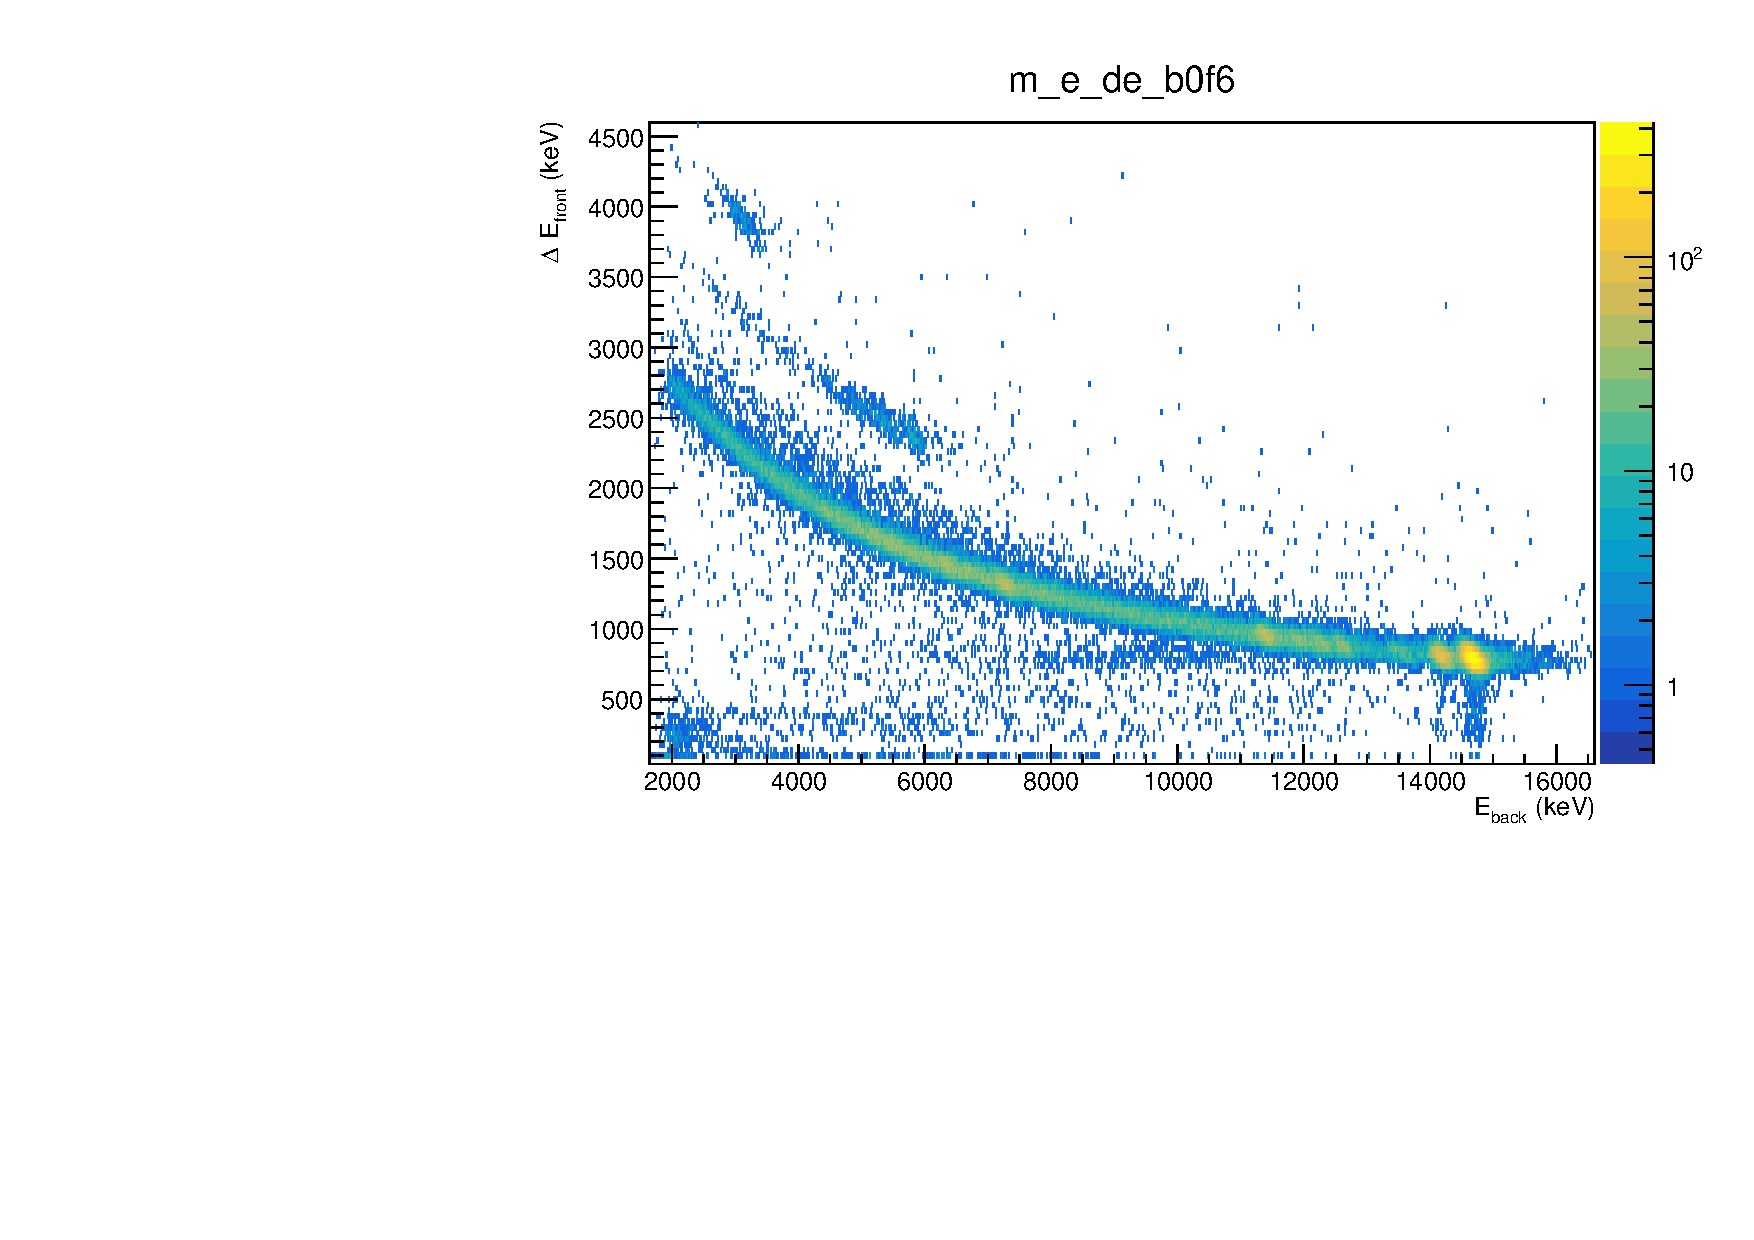
\includegraphics[width=0.6\linewidth]{figures/m_e_de_b0f6_calibrated.pdf}
    \caption{Calibrated $E\Delta E$ plot for \nuclide[106]{Pd}. The top banana observed at $\Delta E \approx 4000$ keV represents tritons from \nuclide[106]{Pd}$(p,t\gamma)$\nuclide[104]{Pd}. The middle banana at $3500 \text{ keV} < \Delta E < 2000$ keV represents deuterons from \nuclide[106]{Pd}$(p,d\gamma)$\nuclide[105]{Pd}. The bottom banana at  $3000 \text{ keV} < \Delta E < 500$ kev represents \nuclide[106]{Pd}$(p,p'\gamma)$\nuclide[106]{Pd}, which is the particle that is gated for. The related $\gamma$-coincidences are shown in the $\gamma$-energy spectra (\cref{fig:106Pd_Eg}) and excitation matrices (\cref{fig:Ex_Eg})}
    \label{fig:106Pd_EdE}
\end{figure}
% \subsubsection{EdE}


\begin{figure}
    \centering
    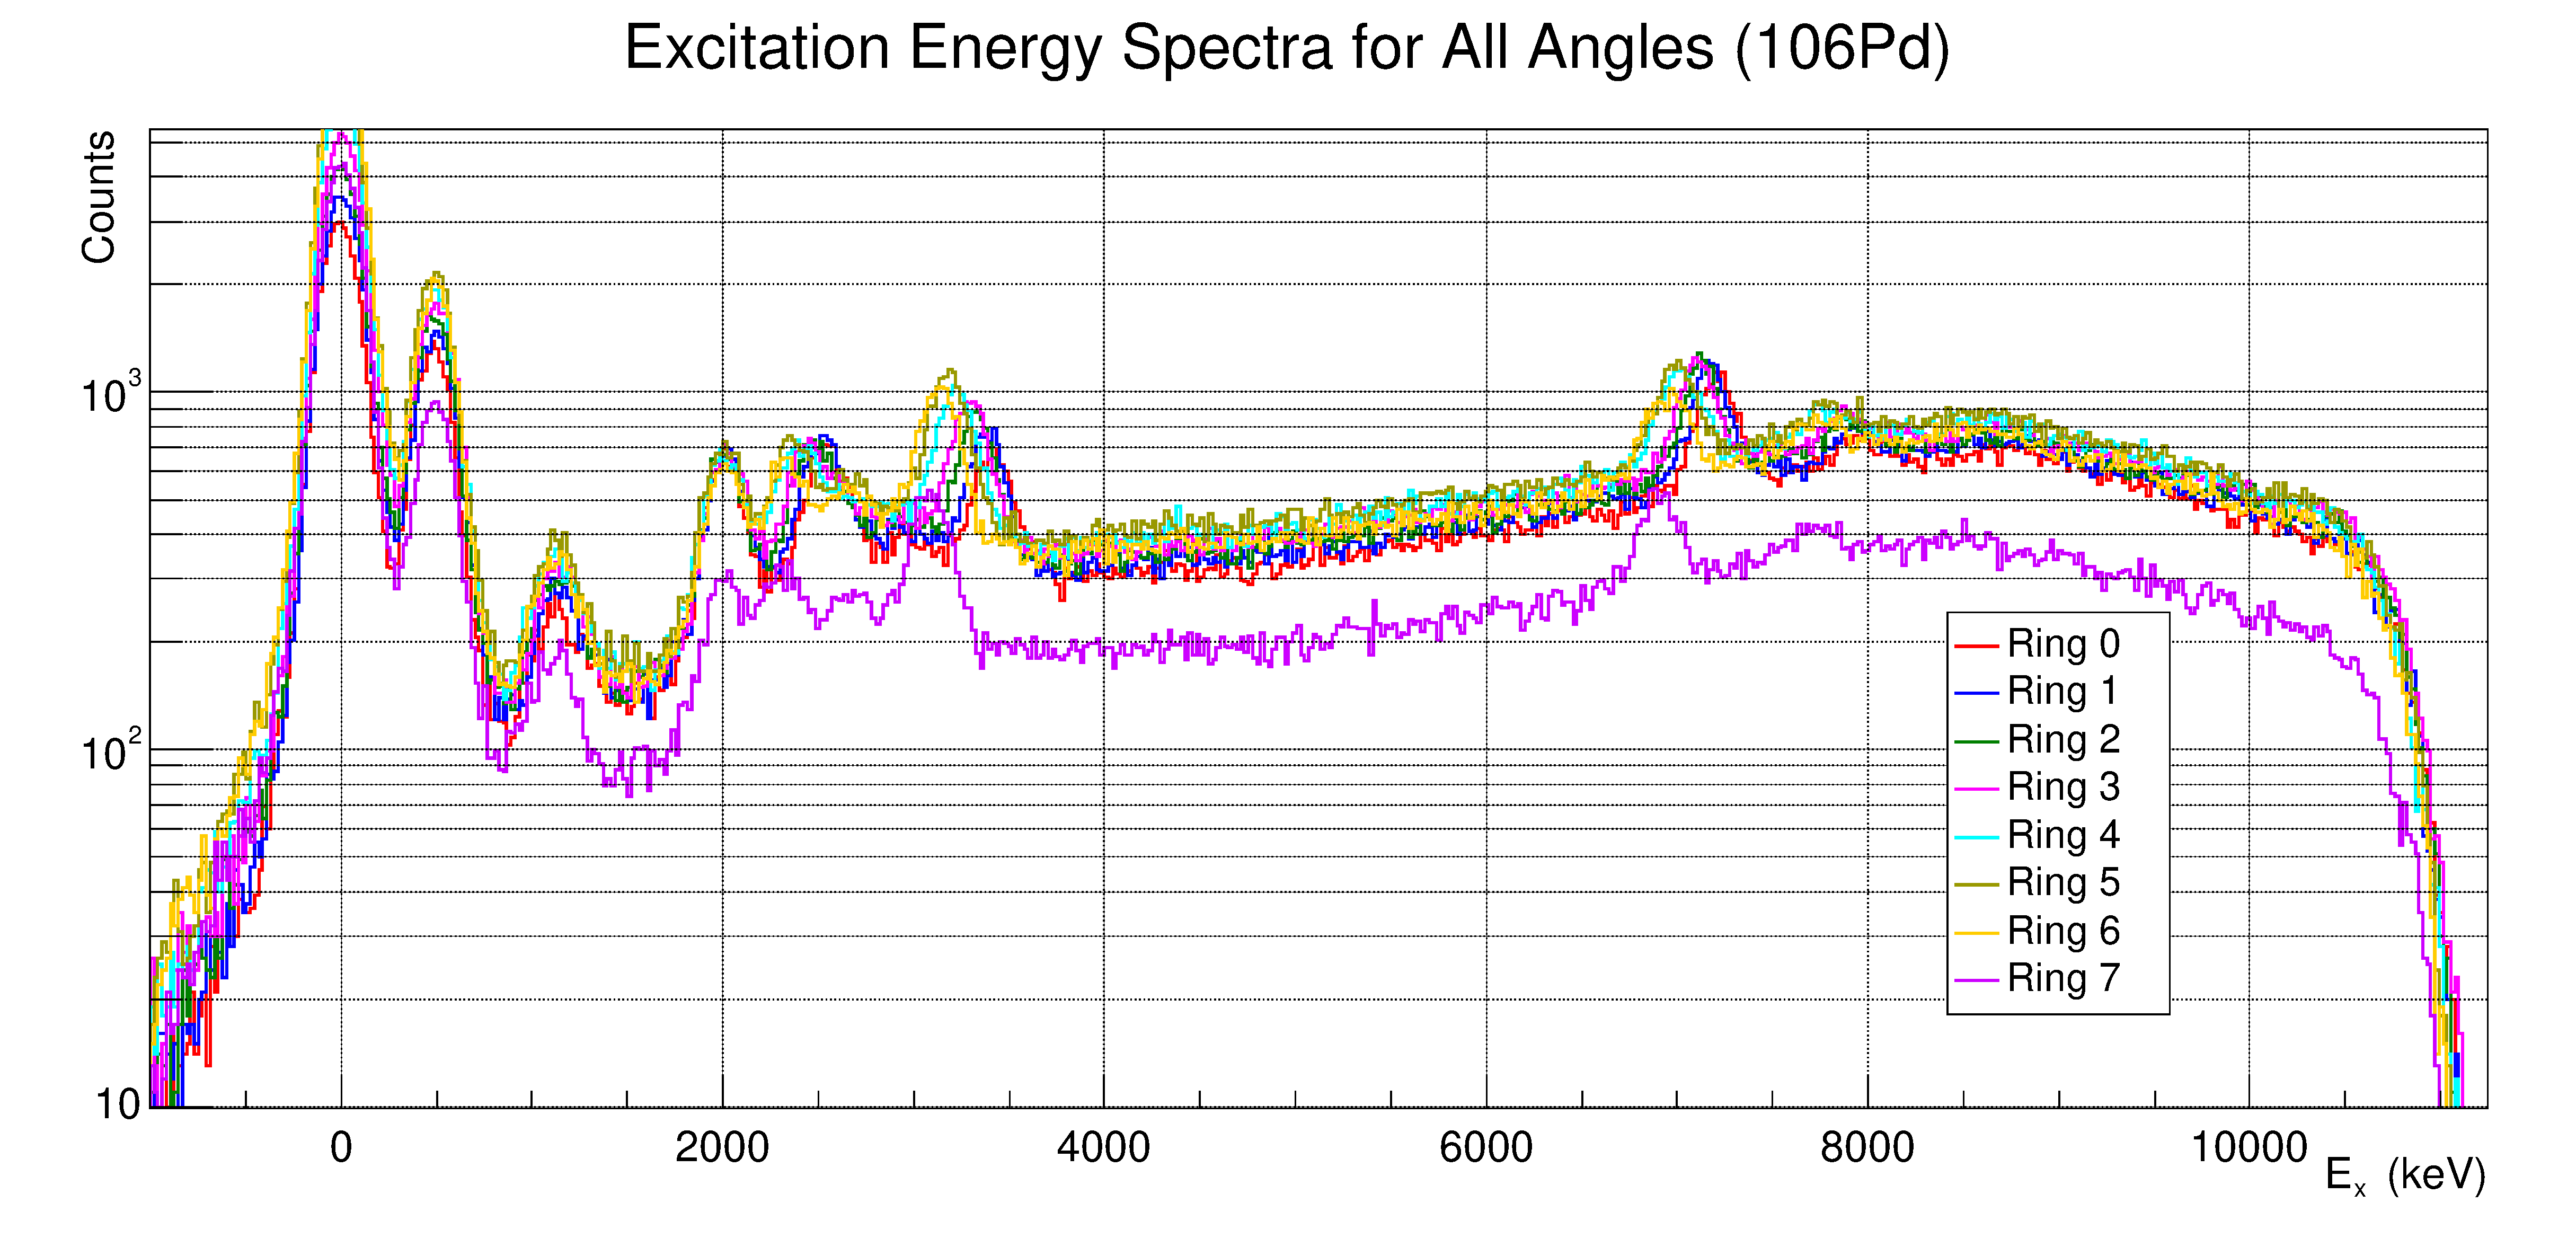
\includegraphics[width=0.9\linewidth]{figures/Ex_energies_106Pd.pdf}
    \caption{The excitation spectra for \nuclide[106]{Pd} where protons have been gated for. The lowest excitation level has been aligned at 0 keV, where tops are graphically excluded in this figure to show smaller details. Ring 7 contains significantly lower amounts as a result of f7 often giving unusable data. As the excitation energies increase, pollutants such as carbon and oxygen show up. These are misaligned to each other, as the lowest excitations of \nuclide[106]{Pd} were used in the alignment. Each bin on the x-axis represents 20 keV.}
    \label{fig:106Pd_Ex}
\end{figure}
The excitation energies of each calibrated ring of SiRi for the \nuclide[106]{Pd}$(p,p'\gamma)$\nuclide[106]{Pd} are shown in \cref{fig:106Pd_Ex}, where ground state is clearly aligned at 0 keV. The spectra contains energies corresponding 
At above $\sim 2$ MeV, the peaks become less aligned, as they represent pollutants to some extent. Observed excitation energies at $\sim 500$ keV,  $\sim 1130$ keV,  $\sim 2010$ keV, with several excitation energies above this which are harder to comfortably determine. Due to SiRi's energy resolution of 150 keV, cleanly determining levels is tough. In perspective of the strong peaks of $\gamma$-energy spectra of \nuclide[106]{Pd}, the first two excitation energies likely correspond to levels 511.85 keV, 1229.30 keV. The highest excitation energy prominently observed is at $\sim 7.7$ keV, after the taller peak at $\sim6.8$ keV. 

% \Cref{fig:106Pd_Ex} shows the excitation energies of \nuclide[106]{Pd}, where the peak of most importance at 0 keV is clearly aligned. Later peaks are somewhat skewed and a result of pollutants in the sample (?). The counts from ring 7 are much lower, following that many of the SiRi combinations including the outermost strip were removed. We also observe that the 511's from +1022 keV $\gamma$'s are piling on top of the 2+ level of 511.850 keV \cite{106Pd}.


\subsection{Excitation matrix}
Finally we come to the star of the project, the excitation energy vs. gamma energy matrix (\cref{fig:Ex_Eg}). The matrix has a mostly triangular shape, with exception to low excitation levels. Prominent features can be observed at several points, corresponding to the already mentioned $\gamma$-energies and proton energies. Towards the top right of the plot where we approach higher energy values, the statistics are low. Above 7 MeV excitation energies, counts are bellow 10 despite per bin. 
The background excitation matrix shows prominent features at similar places. Weak horizontal lines can be seen at $E_\gamma$ = 4 MeV, likely corresponding to the \nuclide[27]{Al} frame of the \nuclide[106]{Pd} sample despite being covered with a tantalum layer to reduce interactions with materials of no interest. The counts of the background matrix are 1/10th of that of the excitation matrix.


\begin{figure}[htbp]
    \centering
    \begin{minipage}{0.48\textwidth}
        \centering
        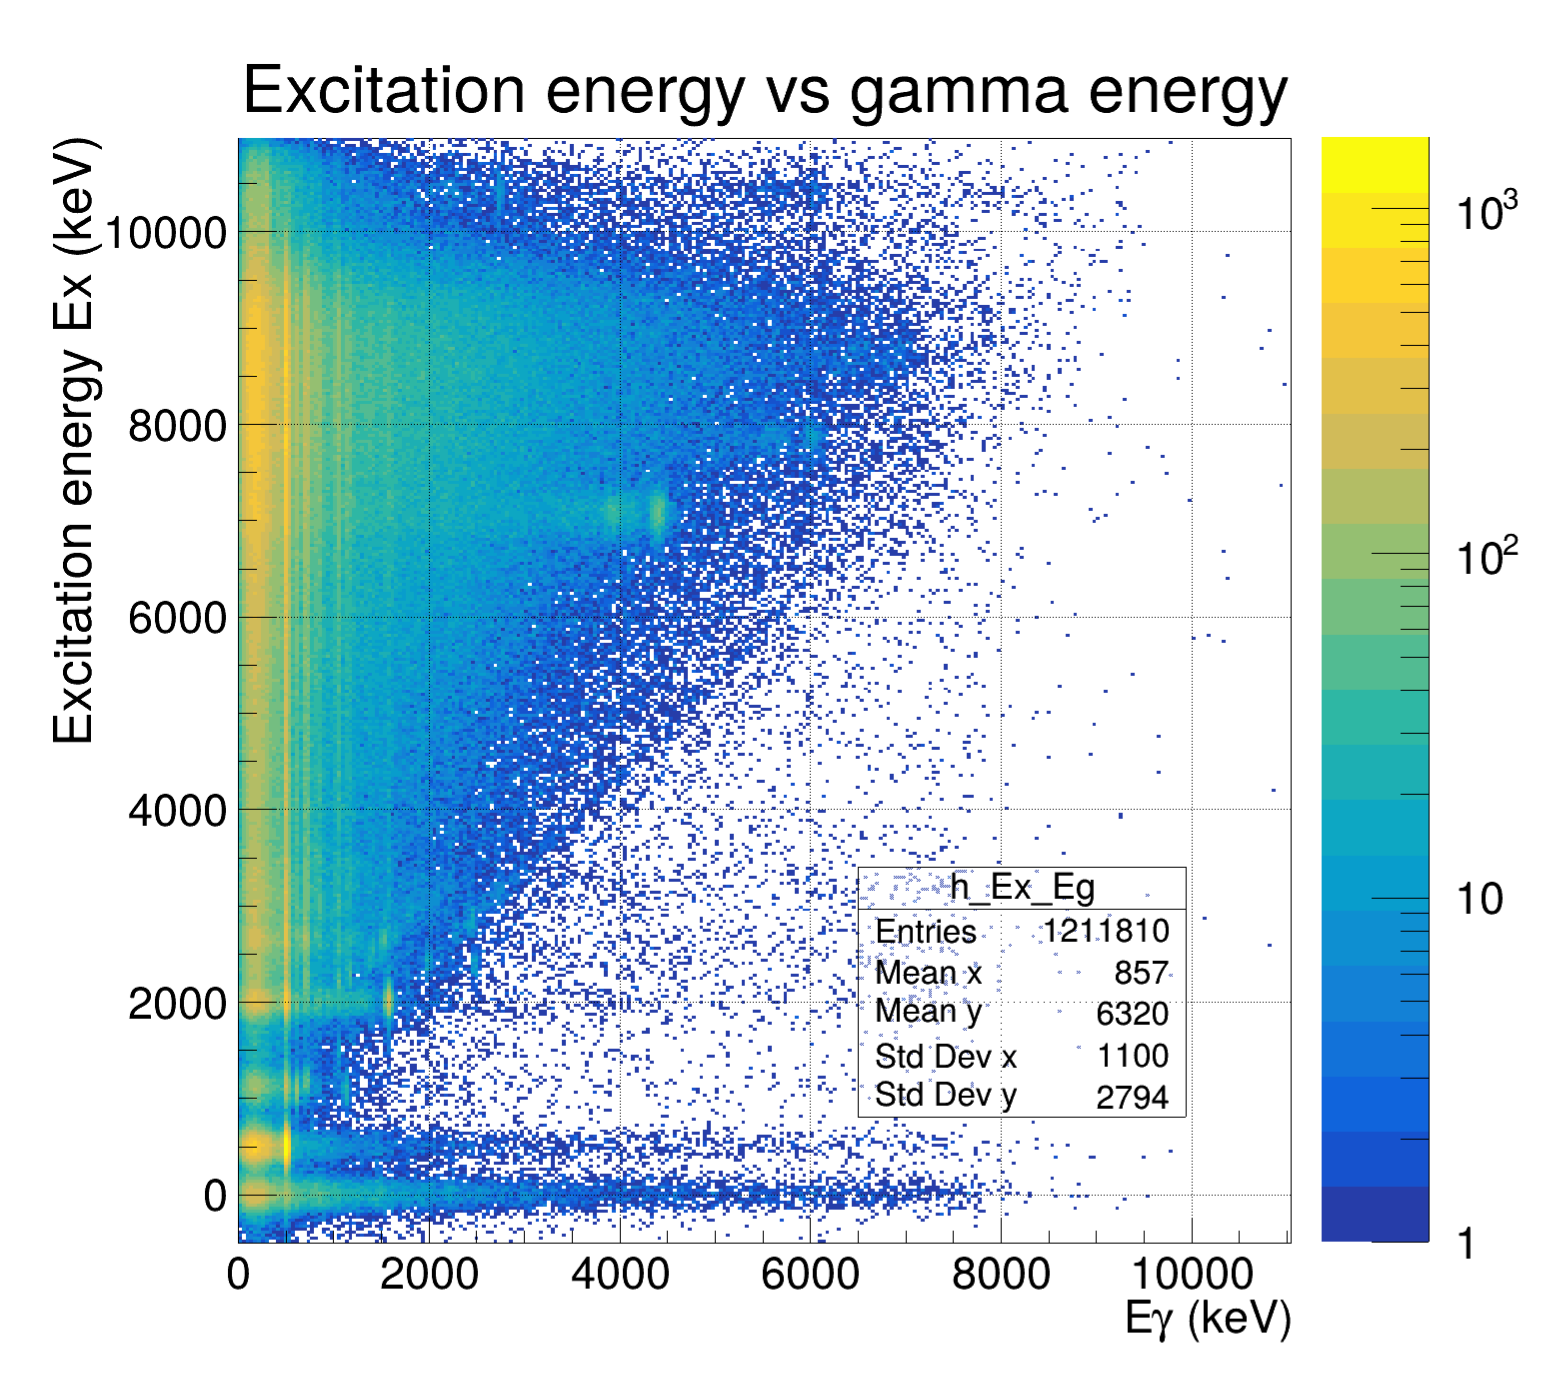
\includegraphics[width=\linewidth]{figures/h_Ex_Eg.png}

    \end{minipage}
    \hfill
    \begin{minipage}{0.48\textwidth}
        \centering
        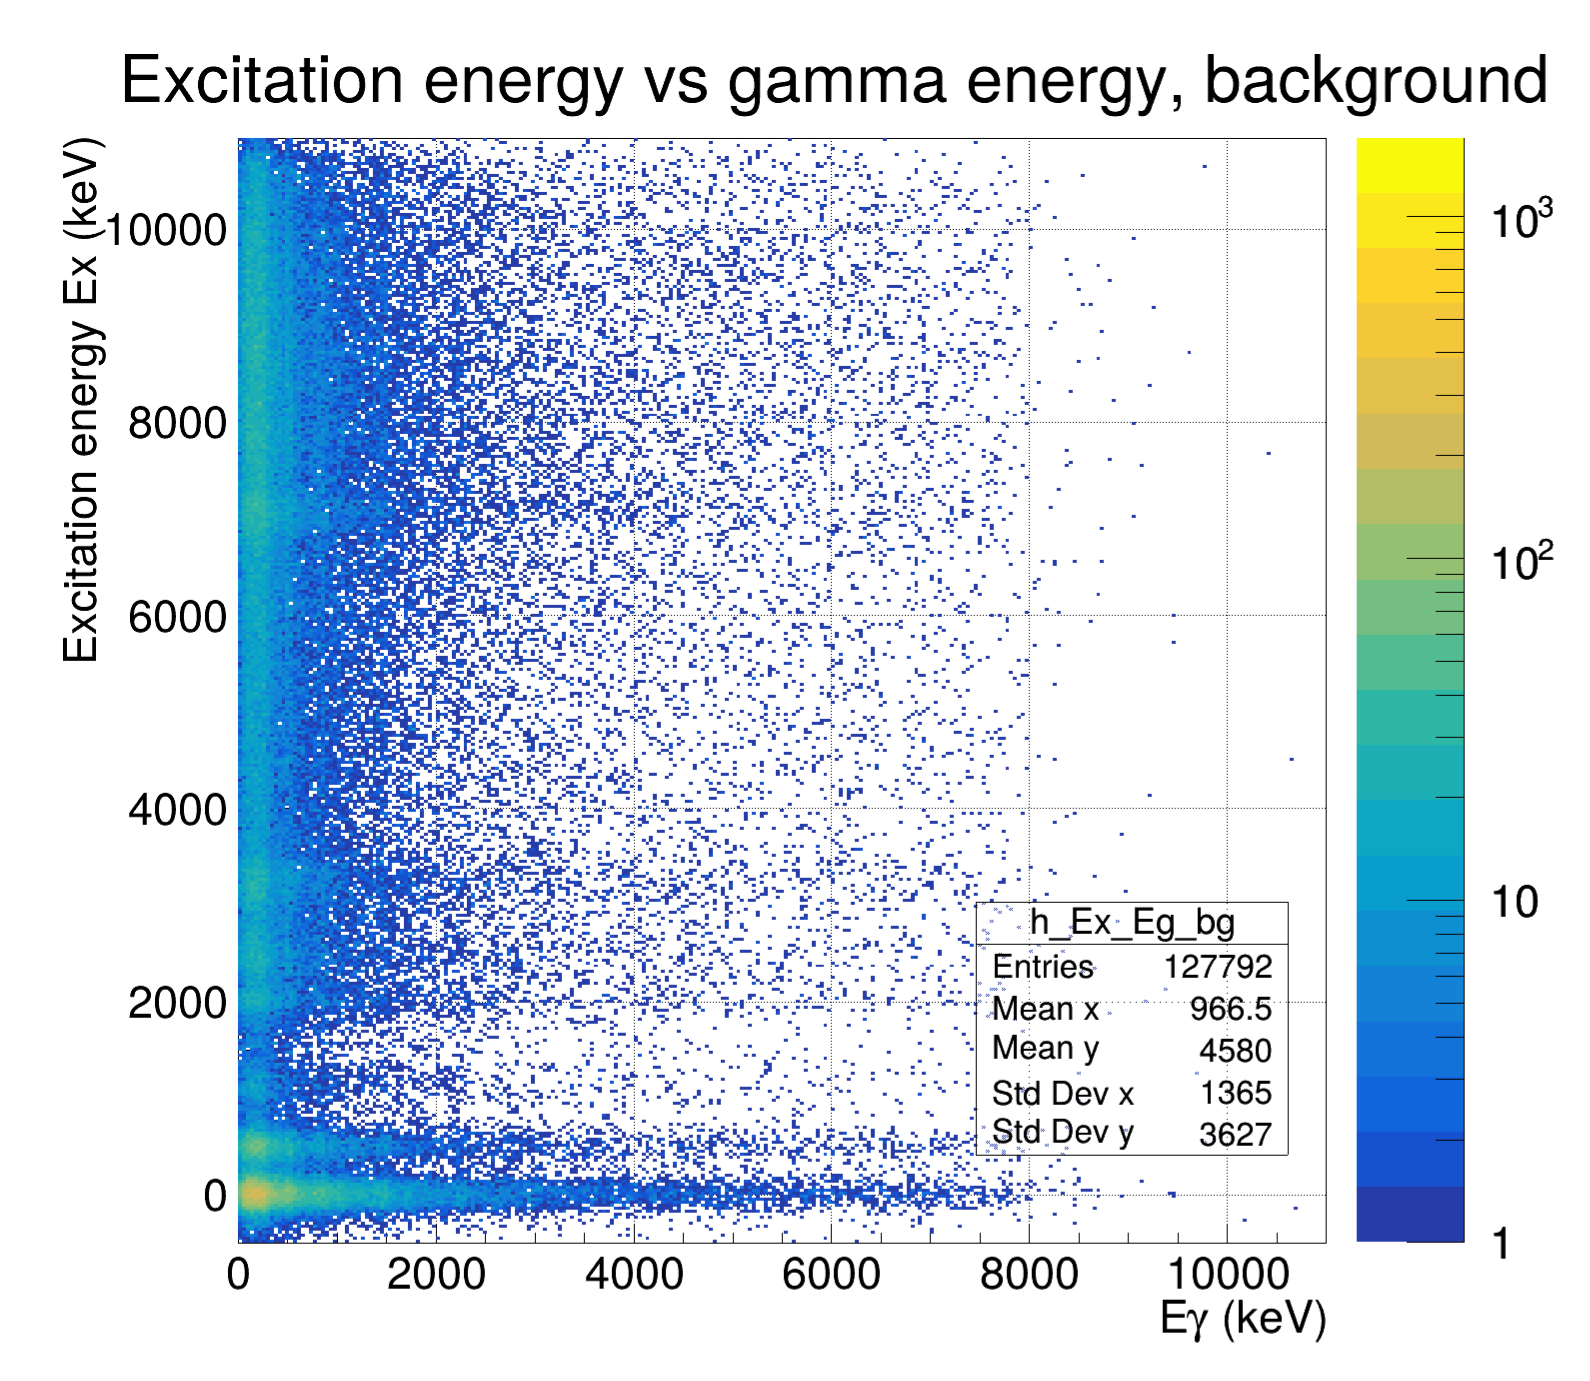
\includegraphics[width=\linewidth]{figures/h_Ex_Eg_bg.png}

    \end{minipage}
    \caption{The figures show the excitation matrices for \nuclide[106]{Pd} and background to the left and right respectively. The excitation matrix has about 10 times more counts than the background matrix. In the background matrix we observe contamination from the aluminum frame of the \nuclide[106]{Pd} target}
    \label{fig:Ex_Eg}
\end{figure}







\newpage
\section{Discussion}
The fitted calibrated $\gamma$-energies of both \nuclide[106]{Pd} and \nuclide[27]{Al} deviated somewhat from the database energies \cite{104Pd,105Pd,106Pd,27Al} by up to 7 keV (\cref{tab:106Pd-fits,tab:27Al-combined-fits,tab:27Al-det1-fits}). This could lead to inaccuracies when the excitation matrix is processed using the OSLO-method. Though, seeing as each SiRi bin spans 20 keV while an OSCAR bin spans 2 keV, a 7 keV deviation may not be of as much importance. Metrics important to the OSLO-method are unclear, consequently aspects not known to the student may have been accidentally disregarded or missed. Regardless, a three point calibration would have improved the $\gamma$-energy calibration results. 

Additionally, neither OSCAR nor SiRi were time aligned, both individually within the array and in correspondence to each other. Though the time gates of 220 to 270 ns is appropriate, due to its wide nature background counts may also be included. A time-alignment could more accurately fill the background matrix, needed for later background-removal before use in the OSLO-method. Contamination from the \nuclide[27]{Al} framing of the \nuclide[106]{Pd} sample seems to be present in the background excitation matrix as well, indicating that the \nuclide[181]{Ta} covering was inadequate. How this would complicate the preparation for the OSLO-method is unclear.

Another point of discussion is the prominent features observed in the \nuclide[106]{Pd} $\gamma$-energy spectra observed at $\sim4.4$ MeV and $\sim6$MeV. These are not present in the databases for \nuclide[104]{Pd}, \nuclide[105]{Pd} or \nuclide[105]{Pd} \cite{104Pd,105Pd,106Pd}, but $\gamma$-decay energies in these ranges for \nuclide[27]{Al} are present in the database (\cite{27Al}). Though when investigating if these features are present in collected proton gates spectra, the answer is not to such an extent (see \cref{fig:27Al-energy-whole}). If the \nuclide[106]{Pd} $\gamma$-energy spectra was contaminated by the aluminum frame, one would expect similar features to appear at the same energies, but so seems not to be the case. This is worth further investigating to unveil the origin of the energy peaks. 

As seen in \cref{fig:excitation-shift}, the SiRi detector segments experienced a slight shift in excitation energies to the left. The \textsc{Qkinz} calculations for \nuclide[106]{Pd} assumed a perfect detector with no dead layer. It seems this was not appropriate, but was easily corrected for by applying a shift to the rings of SiRi. 

Several of the detectors, both for SiRi and OSCAR, gave bad data. 13 SiRi combinations experienced a downwards shift, and 3 OSCAR detectors gave unreasonably large FHWMs(\cref{fig:LaBr3-bad-detectors}) with unresolvable peaks in otherwise resolvable areas. Otherwise, OSCAR detector resolutions ranged between 5 \% to 11 \% at 511 keV, despite supposedly being able to achieve 2.7\%-4.3\% at 662 keV. The necessary removal of 17\% of the detectors due to technical issues, the overall counts are lessened and statistics are worsened.  

The excitation energy spectra (\cref{fig:106Pd_Ex}) supposedly contains pollutants such as oxygen and carbon. To what point these play part in the excitation matrix, and which peaks these correspond to is unclear. 

\begin{figure}
    \begin{minipage}{0.45\textwidth}
        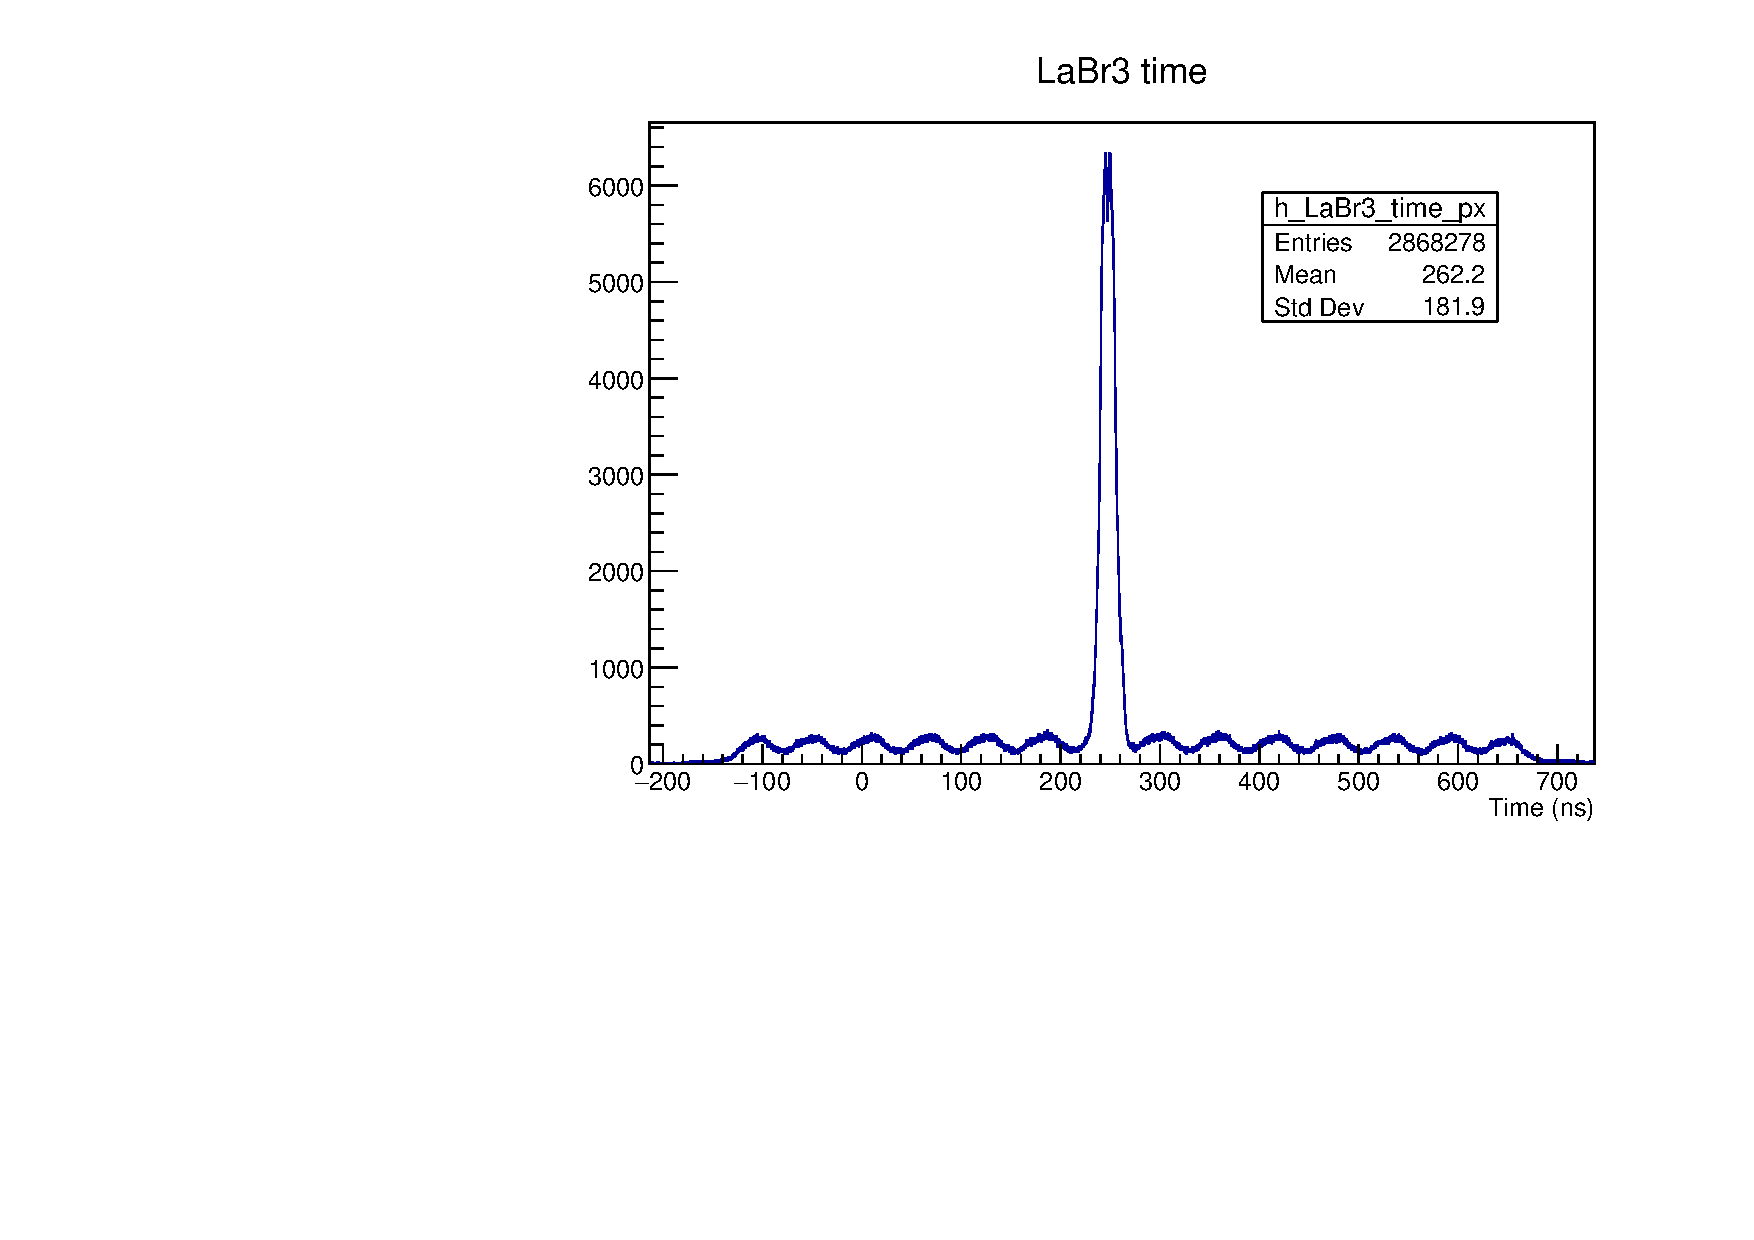
\includegraphics[width=1\linewidth]{figures/106Pd_LaBrr3_time.pdf}
    \end{minipage}
    \begin{minipage}{0.45\textwidth}
        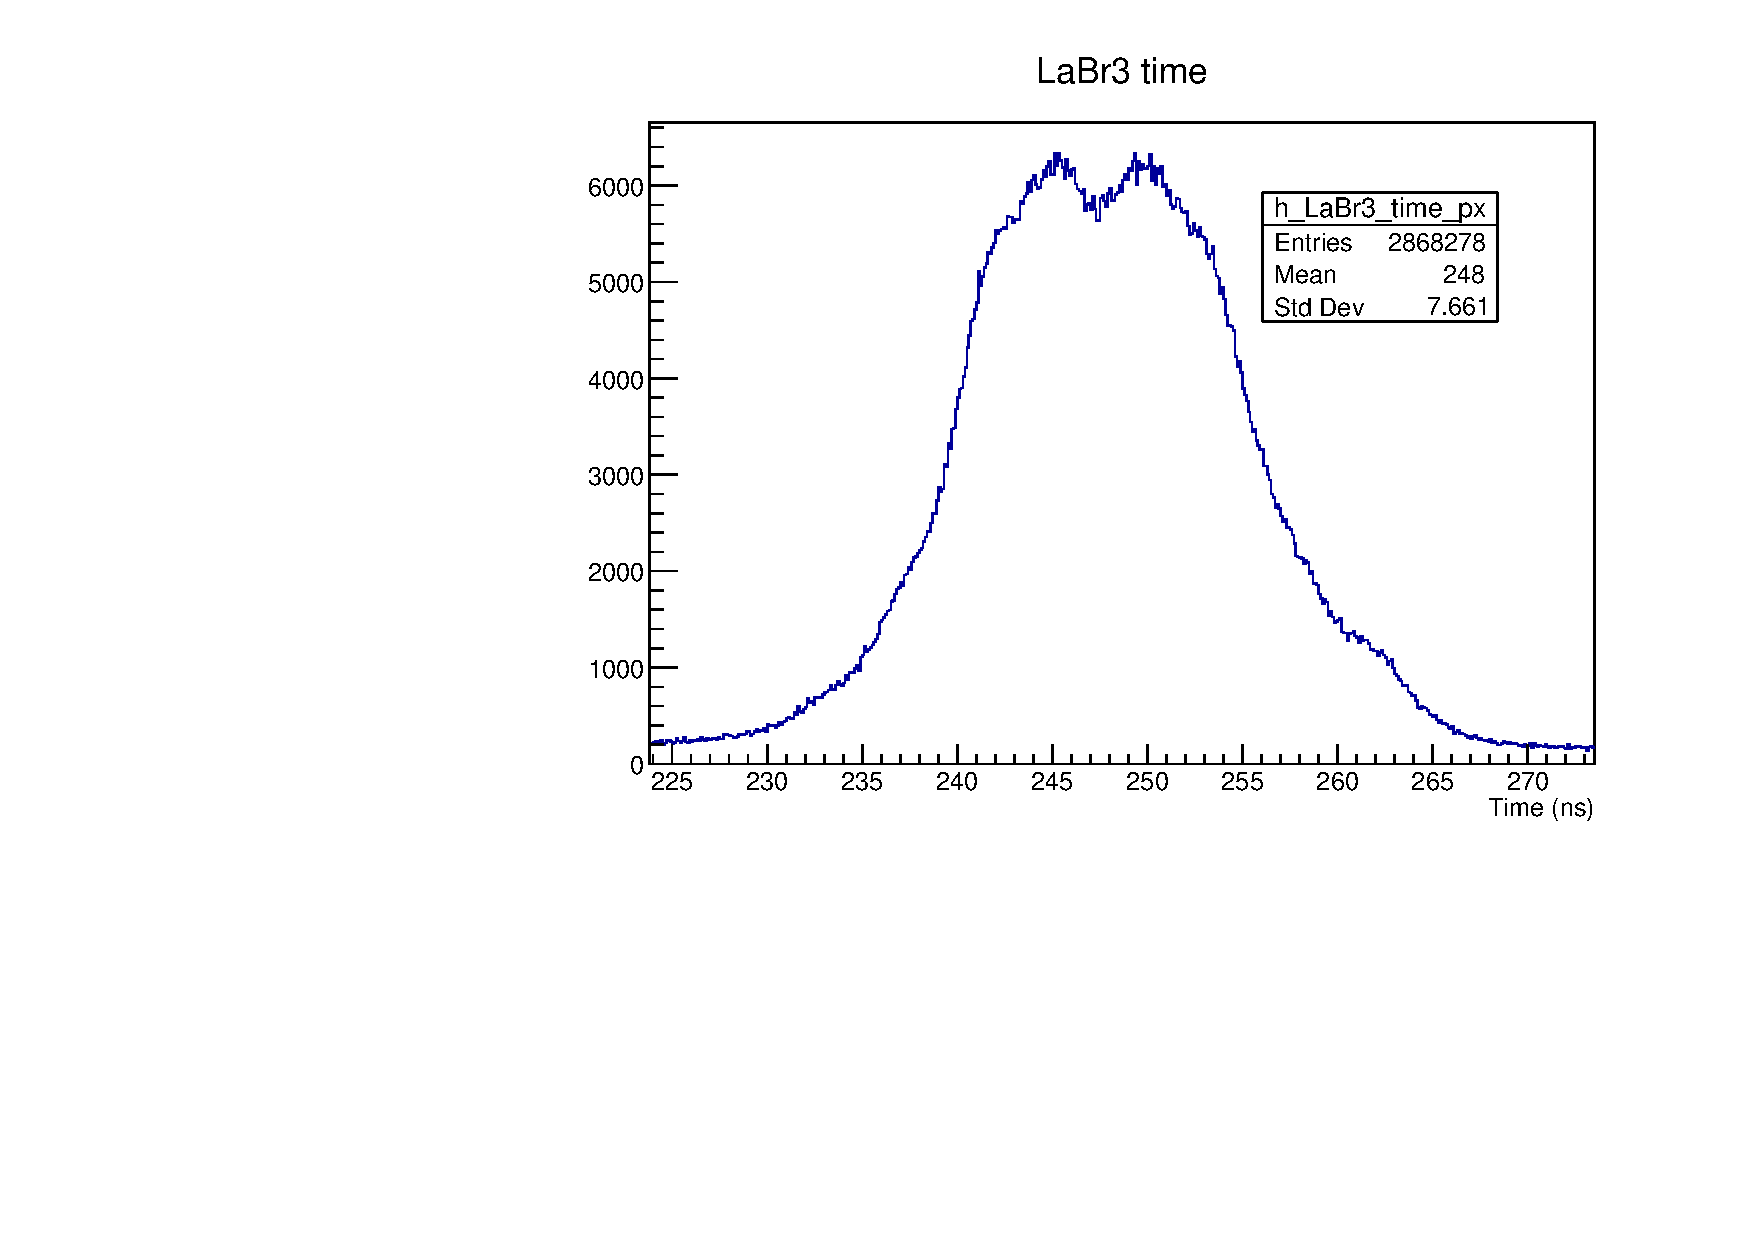
\includegraphics[width=1\linewidth]{figures/106Pd_LaBrr3_time_gated.pdf}
    \end{minipage}
    \centering
    \caption{Figures showing the time misalignment of \nuclide[106]{Pd}. The figure to the right shows that the tops are misaligned.}
    \label{fig:106Pd-time}
\end{figure}

\newpage
\section{Conclusion}
The excitation vs gamma energy matrix (\cref{fig:Ex_Eg}) for the \nuclide[106]{Pd}$(p,p'\gamma)$\nuclide[106]{Pd} reaction was acquired through proper gain-matching. Excitation energies were collected and calibrated for and with \nuclide[106]{Pd} with \textsc{Qkinz} calculations. Gamma energies were calibrated and acquired for \nuclide[27]{Al} with the purpose of calibrating \nuclide[106]{Pd}, in agreement with database values, but with deviation up to 7 keV for inspected peaks.
The background excitation vs gamma energy matrix was constructed, containing about 1/10th of the counts as the main matrix. Contaminants of \nuclide[27]{Al} interactions may be present.

Both excitation vs gamma energy matrices are affected by not time-aligning OSCAR and SiRi. Future work should address this, hopefully restricting the matrices in preparations for OSLO-method applications.  

The $\gamma$-energy spectra for \nuclide[106]{Pd} showed prominent structures at $\sim4.4$ MeV and $\sim6$ MeV despite databases for \nuclide[104]{Pd}, \nuclide[105]{Pd} and \nuclide[106]{Pd} not featuring such energies. It seems the \nuclide[27]{Al} frame isn't the culprit either. Identifying the origin of the structures would be cool.

\section{Declaration of generative AI use}
LLMs were used as an assistance in coding and understanding ROOT, as neither ROOT nor C++ were familiar. For this, both Claude Sonnet and Claude Haiku were used. This mostly concerns understanding code, making plotting functions. The process of calibration itself was not tweaked using LLMs. UiO GPT-5.1 Thinking and Claude Sonnet were used for latex table and image layout tweaking. No LLMs were used in writing, typesetting and proofreading of the project report.

\newpage
\bibliography{references}

\newpage
\appendix
\section{OSCAR}

\begin{table}[htbp]
    \centering
    \begin{minipage}{0.50\textwidth}
        \caption{\nuclide[27]{Al} Gaussian fit results for combined spectra}
        \centering
        \begin{tabular}{ c | c  c  |c }
        \toprule
        {Actual (keV)} & {Mean (keV)} & {$\sigma$ (keV)} & {$\chi^2$/NDF} \\
        \midrule
       511.00  & $511.1 \pm 0.0$ & $20.6 \pm 0.0$ & 76.6 \\
       2212.01 & $2219.3 \pm 0.1$ & $29.7 \pm 0.1$ & 13.8 \\
       3004.20 & $3004.9 \pm 0.1$ & $34.5 \pm 0.1$ & 5.9 \\
        \bottomrule
        \end{tabular}
        \label{tab:27Al-combined-fits}
    \end{minipage}%
    \hfill\hfill
    \begin{minipage}{0.45\textwidth}
        \centering
        \caption{\nuclide[27]{Al} Gaussian fit results for detector 1}
        \begin{tabular}{  c  |c c}
            \toprule
            {Mean (keV)} & {$\sigma$ (keV)} & {$\chi^2$/NDF} \\
            \midrule
           $510.9 \pm 0.0$ & $14.3 \pm 0.1$ & 5.6 \\
           $2217.2 \pm 0.2$ & $24.9 \pm 0.3$ & 1.6 \\
           $3009.4 \pm 0.4$ & $29.6 \pm 0.5$ & 2.3 \\
            \bottomrule
        \end{tabular}
        \label{tab:27Al-det1-fits}
        \end{minipage}
        \caption{Calibration is seen to be quite accurate. In these fits, background was not accounted for. The fits accuracy is seen to be poor as  the $\chi^2$/NDF-values are high, especially for the combined energy spectra. The $\sigma$ values are smaller for individual spectra, meaning the combined values must be smeared, giving less accurate results. Time-aligning the LaBr$_3$ measurements could lessen this effect.}
\end{table}

\begin{table}[htbp]
    \centering 
    \caption{\nuclide[106]{Pd}(p,p'$\gamma$) Gaussian fit results. Note that datasheets(\cite{104Pd,105Pd,106Pd}) for \nuclide[104]{Pd}, \nuclide[105]{Pd} and \nuclide[106]{Pd} don't contain $E_\gamma$-transitions that correspond to the 4404 keV and 6034 keV measurement. At this point as seen on the corresponding spectrogram, the statistics are somewhat low so the fits are likely inaccurate. The datasheets however do not contain transitions above 3.2 MeV. The peaks of 1045 and 1050 keV aren't separately resolvable.}
    \begin{tabular}{c c c |c}
        \toprule
        {Adopted (keV)} & {Mean (keV)} & {$\sigma$ (keV)} & {$\chi^2$/NDF} \\
        \midrule
        511.85 & $510.87 \pm 0.05$  & $15.54 \pm 0.06$  & 15.3 \\
        621.9 & $616.85 \pm 0.22$  & $27.26 \pm 0.40$  & 2.9 \\
        717.24 & $719.11 \pm 0.12$  & $18.52 \pm 0.18$  & 2.1 \\
        1045.83 and 1050.39 & $1050.20 \pm 0.24$ & $25.60 \pm 0.41$  & 2.1 \\
        1572.35 & $1575.20 \pm 0.44$ & $38.33 \pm 0.84$  & 1.8 \\
        ? & $4404.52 \pm 1.83$ & $106.91 \pm 3.01$ & 1.5 \\
        ? & $6034.81 \pm 7.49$ & $148.15 \pm 15.72$ & 1.0 \\
        \bottomrule
    \end{tabular}
    \label{tab:106Pd-fits}
\end{table}

\begin{figure}[htbp]
    \centering
    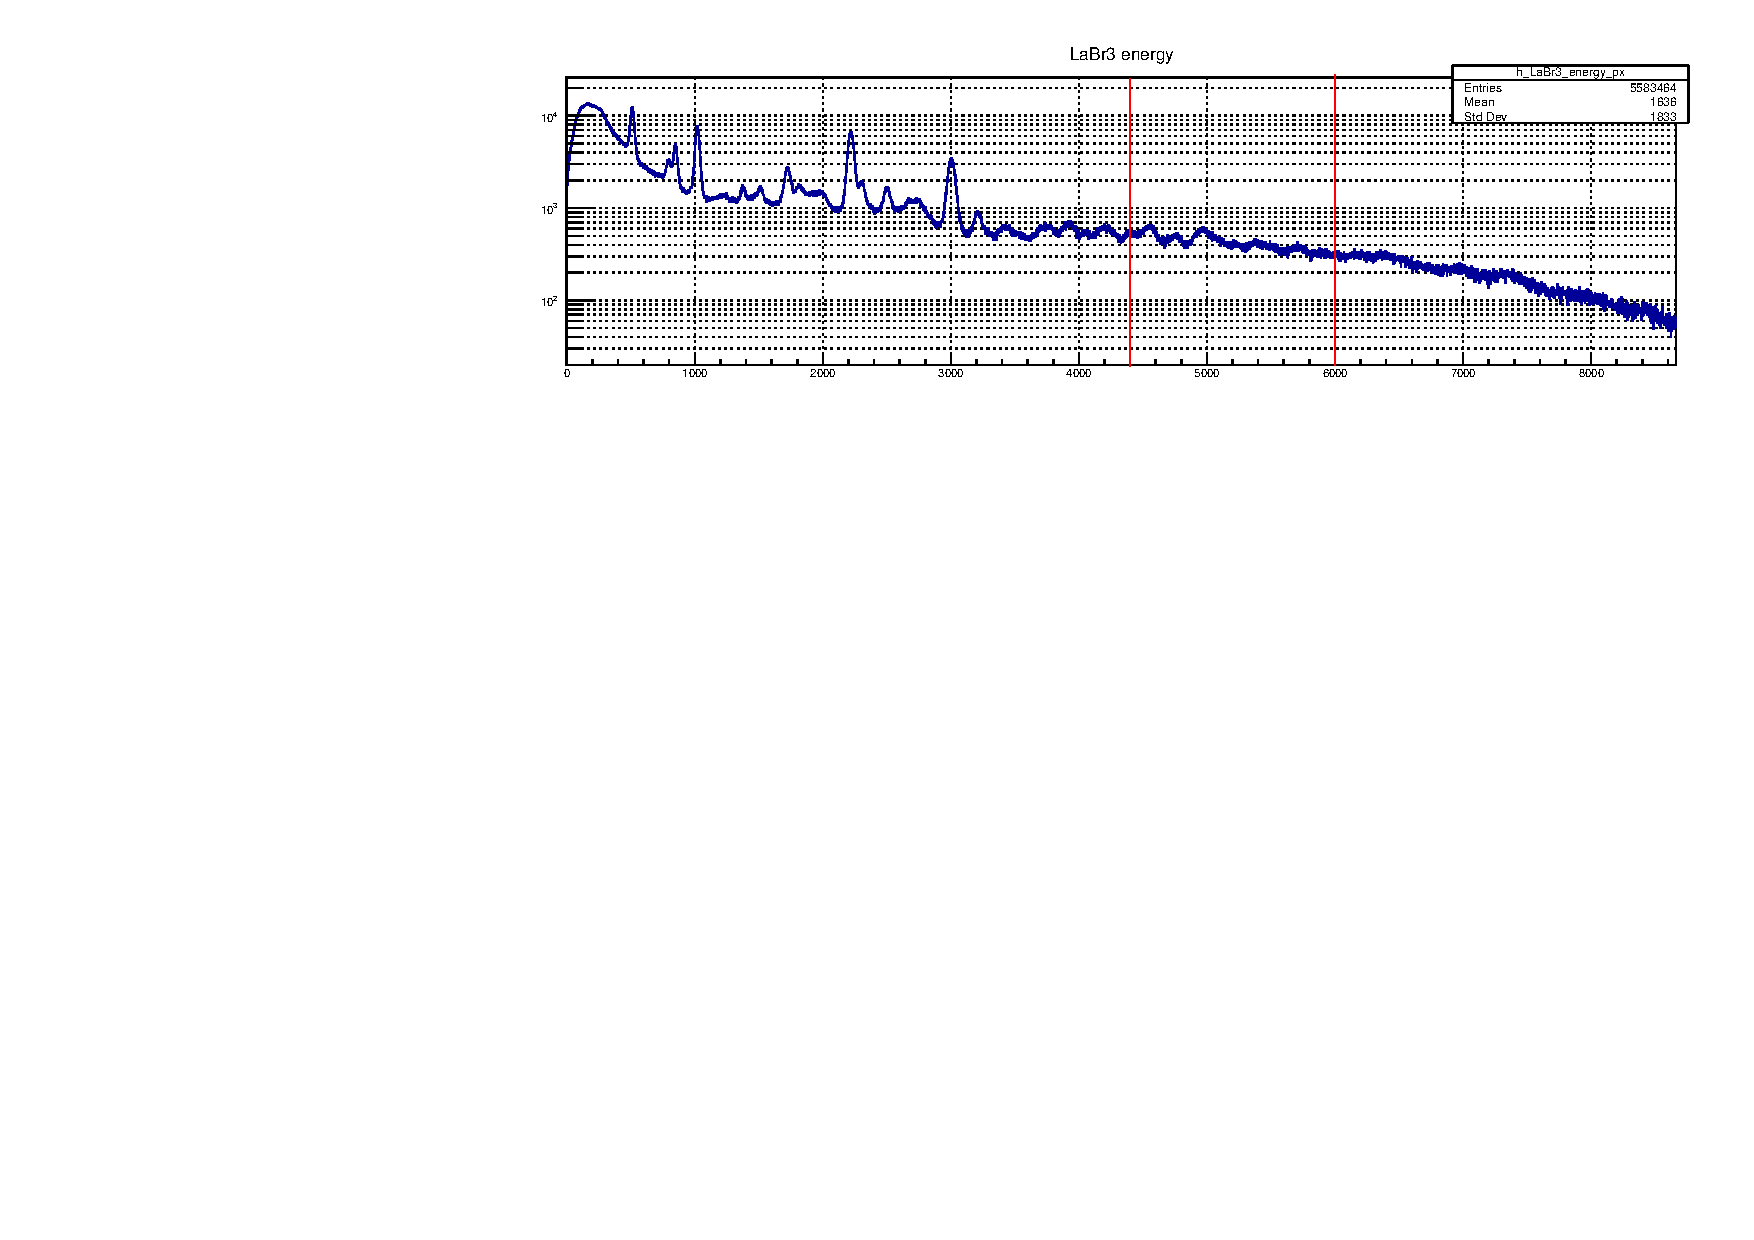
\includegraphics[width=1\linewidth]{figures/27Al_energy_whole.pdf}
    \caption{The $\gamma$-energy spectra of proton gated \nuclide[27]{Al}. No prominent features at $\sim4.4$ MeV and $\sim 6$ MeV of the proportion seen in the $\gamma$-energy spectrum for \nuclide[106]{Pd} are present. }
    \label{fig:27Al-energy-whole}
\end{figure}

\begin{figure}[htbp]
    \centering
    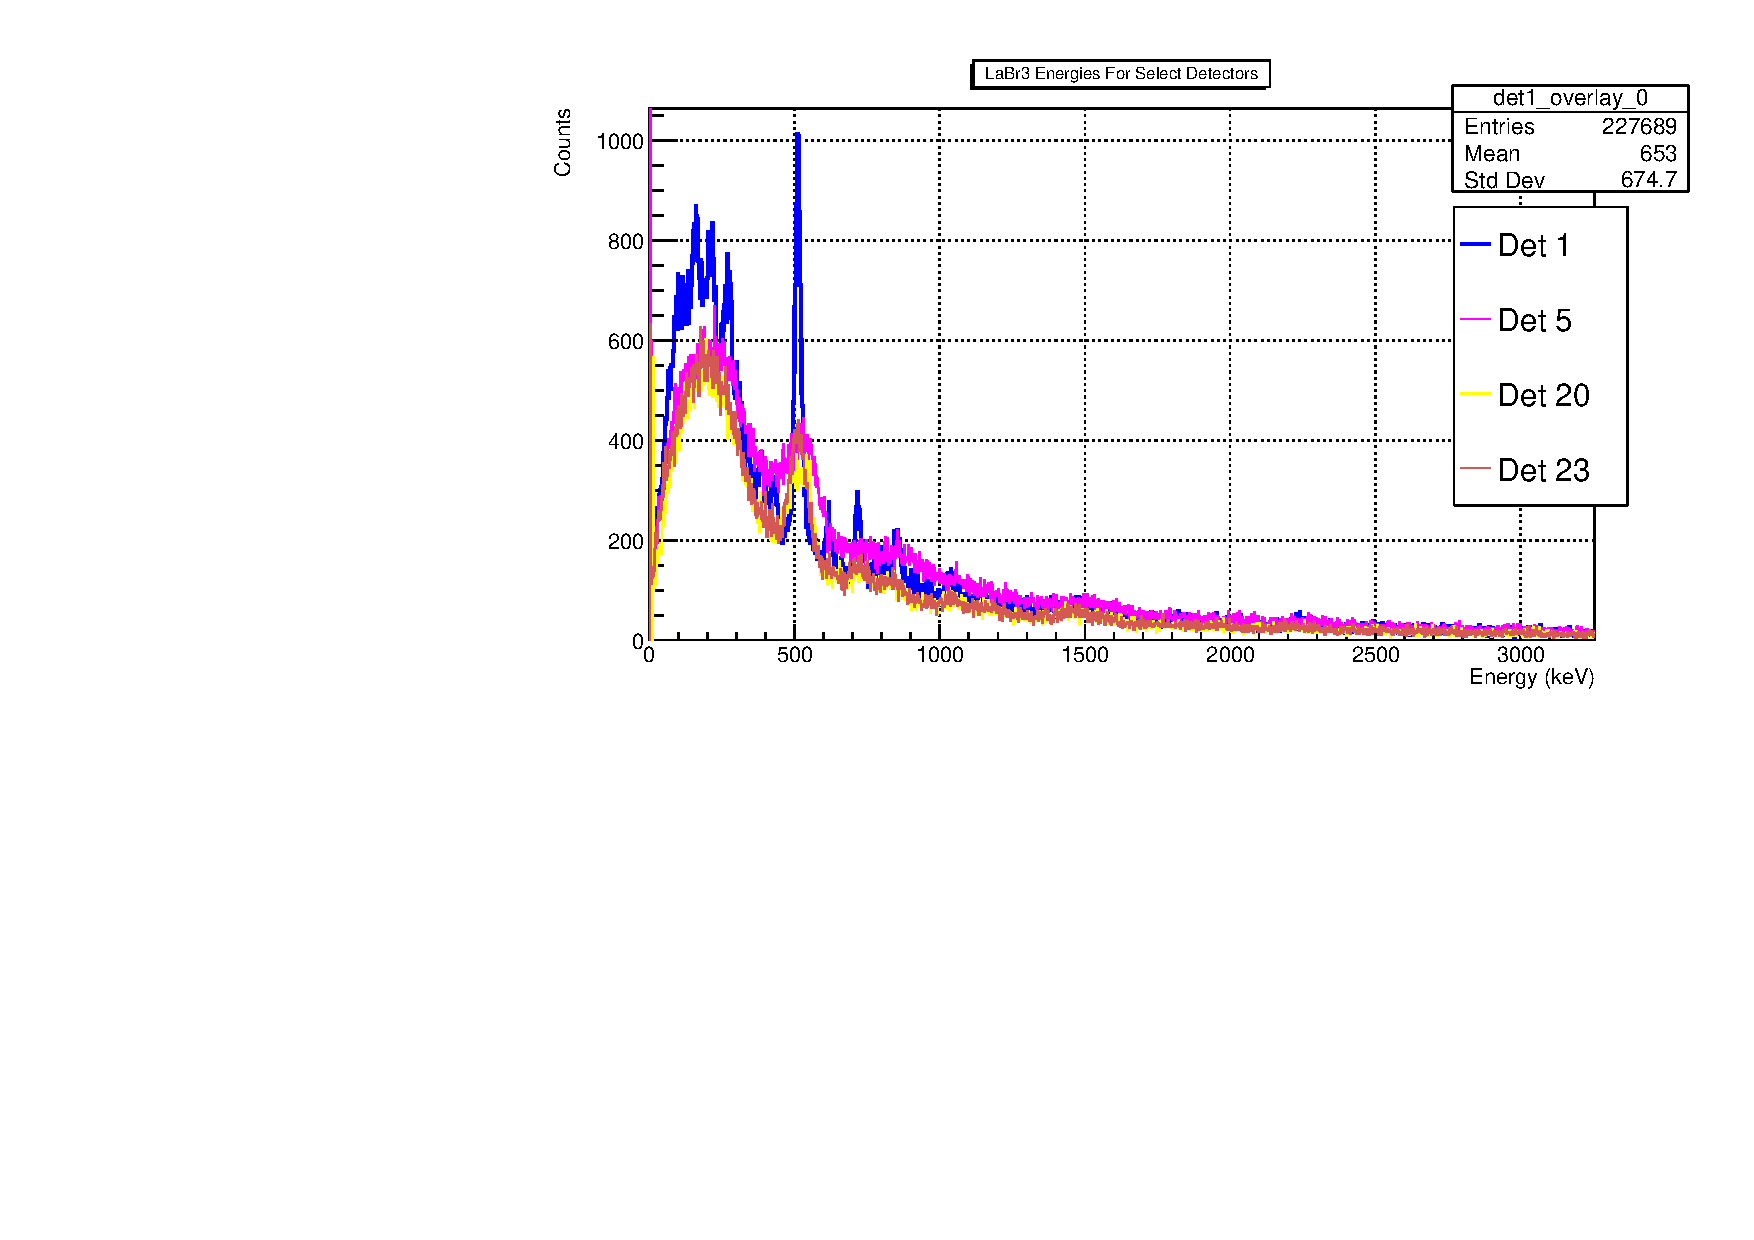
\includegraphics[width=1\linewidth]{figures/LaBr3_energies_1_5_20_23.pdf}
    \caption{Comparison of LaBr3 detector 1 which has good resolution, to detectors 5, 20 and 23 which are to be removed.}
    \label{fig:LaBr3-bad-detectors}
\end{figure}




\newpage
\section{Dataprocessing flowchart}

\begin{figure}[hbt]
    \centering
    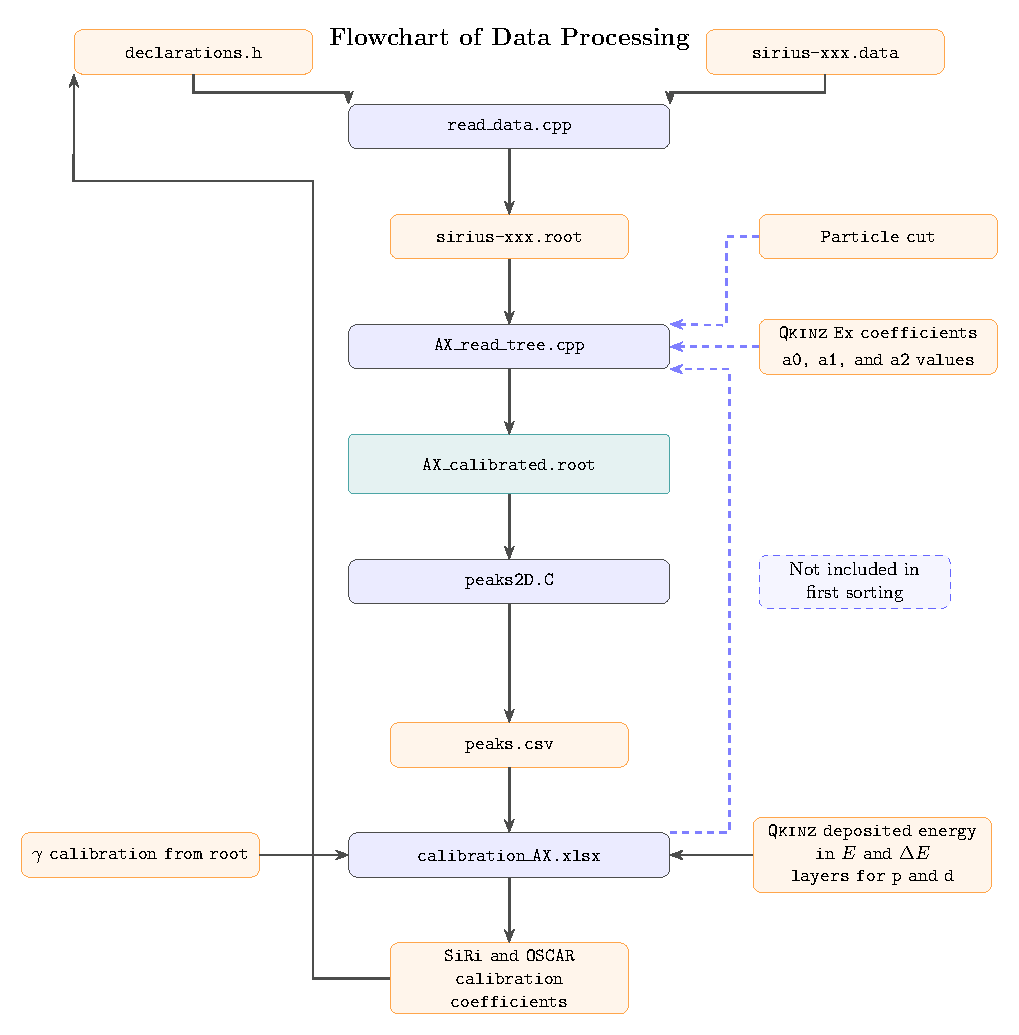
\includegraphics[width=0.8\linewidth]{figures/FYS2810-flowchart.pdf}
    \caption{Calibration of both OSCAR and SiRi is an iterative process. The AX\_calibrated.root is the end file when calibrations are done, where figures can be made from the data.}
    \label{fig:flowchart}
\end{figure}

\end{document}
